% **************************************************************************************************************
% A Classic Thesis Style
% An Homage to The Elements of Typographic Style
%
% Copyright (C) 2015 André Miede http://www.miede.de
%
% If you like the style then I would appreciate a postcard. My address
% can be found in the file ClassicThesis.pdf. A collection of the
% postcards I received so far is available online at
% http://postcards.miede.de
%
% License:
% This program is free software; you can redistribute it and/or modify
% it under the terms of the GNU General Public License as published by
% the Free Software Foundation; either version 2 of the License, or
% (at your option) any later version.
%
% This program is distributed in the hope that it will be useful,
% but WITHOUT ANY WARRANTY; without even the implied warranty of
% MERCHANTABILITY or FITNESS FOR A PARTICULAR PURPOSE.  See the
% GNU General Public License for more details.
%
% You should have received a copy of the GNU General Public License
% along with this program; see the file COPYING.  If not, write to
% the Free Software Foundation, Inc., 59 Temple Place - Suite 330,
% Boston, MA 02111-1307, USA.
%
% **************************************************************************************************************
\RequirePackage{fix-cm} % fix some latex issues see: http://texdoc.net/texmf-dist/doc/latex/base/fixltx2e.pdf
\documentclass[ article,titlepage,numbers=noenddot,headinclude,%1headlines,% letterpaper a4paper
                footinclude=true,cleardoublepage=empty,abstractoff, % <--- obsolete, remove (todo)
                BCOR=5mm,paper=a4,fontsize=12pt,%13pt,a4paper,%
                ngerman,american,%
                ]{scrreprt}

%********************************************************************
% Note: Make all your adjustments in here
%*******************************************************
% ****************************************************************************************************
% classicthesis-config.tex
% formerly known as loadpackages.sty, classicthesis-ldpkg.sty, and classicthesis-preamble.sty
% Use it at the beginning of your ClassicThesis.tex, or as a LaTeX Preamble
% in your ClassicThesis.{tex,lyx} with % ****************************************************************************************************
% classicthesis-config.tex
% formerly known as loadpackages.sty, classicthesis-ldpkg.sty, and classicthesis-preamble.sty
% Use it at the beginning of your ClassicThesis.tex, or as a LaTeX Preamble
% in your ClassicThesis.{tex,lyx} with % ****************************************************************************************************
% classicthesis-config.tex
% formerly known as loadpackages.sty, classicthesis-ldpkg.sty, and classicthesis-preamble.sty
% Use it at the beginning of your ClassicThesis.tex, or as a LaTeX Preamble
% in your ClassicThesis.{tex,lyx} with \input{classicthesis-config}
% ****************************************************************************************************
% If you like the classicthesis, then I would appreciate a postcard.
% My address can be found in the file ClassicThesis.pdf. A collection
% of the postcards I received so far is available online at
% http://postcards.miede.de
% ****************************************************************************************************


% ****************************************************************************************************
% 0. Set the encoding of your files. UTF-8 is the only sensible encoding nowadays. If you can't read
% äöüßáéçèê∂åëæƒÏ€ then change the encoding setting in your editor, not the line below. If your editor
% does not support utf8 use another editor!
% ****************************************************************************************************
\PassOptionsToPackage{utf8}{inputenc}
	\usepackage{inputenc}

% ****************************************************************************************************
% 1. Configure classicthesis for your needs here, e.g., remove "drafting" below
% in order to deactivate the time-stamp on the pages
% ****************************************************************************************************
\PassOptionsToPackage{eulerchapternumbers,listings,%
					 pdfspacing,%floatperchapter,%linedheaders,%
					 subfig,beramono,eulermath,parts}{classicthesis}
% ********************************************************************
% Available options for classicthesis.sty
% (see ClassicThesis.pdf for more information):
% drafting
% parts nochapters linedheaders
% eulerchapternumbers beramono eulermath pdfspacing minionprospacing
% tocaligned dottedtoc manychapters
% listings floatperchapter subfig
% ********************************************************************


% ****************************************************************************************************
% 2. Personal data and user ad-hoc commands
% ****************************************************************************************************
\newcommand{\myTitle}{Introducción a la Homología Singular. Resolución del problema del clique máximo.\xspace}
%\newcommand{\mySubtitle}{An Homage to The Elements of Typographic Style\xspace}
%\newcommand{\myDegree}{Doktor-Ingenieur (Dr.-Ing.)\xspace}
\newcommand{\myName}{José Carlos Entrena Jiménez\xspace}
\newcommand{\myProf}{Francisco Urbano Pérez-Aranda\xspace}
\newcommand{\myOtherProf}{Salvador García López\xspace}
\newcommand{\mySupervisor}{Put name here\xspace}
\newcommand{\myFaculty}{Put data here\xspace}
\newcommand{\myDepartment}{Put data here\xspace}
\newcommand{\myUni}{Universidad de Granada\xspace}
\newcommand{\myLocation}{Granada\xspace}
\newcommand{\myTime}{Septiembre 2017\xspace}

% ********************************************************************
% Setup, finetuning, and useful commands
% ********************************************************************
\newcounter{dummy} % necessary for correct hyperlinks (to index, bib, etc.)
\newlength{\abcd} % for ab..z string length calculation
\providecommand{\mLyX}{L\kern-.1667em\lower.25em\hbox{Y}\kern-.125emX\@}
\newcommand{\ie}{i.\,e.}
\newcommand{\Ie}{I.\,e.}
\newcommand{\eg}{e.\,g.}
\newcommand{\Eg}{E.\,g.}
% ****************************************************************************************************


% ****************************************************************************************************
% 3. Loading some handy packages
% ****************************************************************************************************
% ********************************************************************
% Packages with options that might require adjustments
% ********************************************************************
%\PassOptionsToPackage{ngerman,american}{babel}   % change this to your language(s)
% Spanish languages need extra options in order to work with this template
\PassOptionsToPackage{spanish,es-lcroman}{babel}
	\usepackage{babel}

\usepackage{csquotes}
\PassOptionsToPackage{%
    %backend=biber, %instead of bibtex
	backend=bibtex8,bibencoding=ascii,%
	language=spanish,%
	style=numeric-comp,%
    %style=authoryear-comp, % Author 1999, 2010
    %bibstyle=authoryear,dashed=false, % dashed: substitute rep. author with ---
    sorting=nyt, % name, year, title
    maxbibnames=10, % default: 3, et al.
    %backref=true,%
    natbib=true % natbib compatibility mode (\citep and \citet still work)
}{biblatex}
    \usepackage{biblatex}

\PassOptionsToPackage{fleqn}{amsmath}       % math environments and more by the AMS
    \usepackage{amsmath}

% ********************************************************************
% General useful packages
% ********************************************************************
\PassOptionsToPackage{T1}{fontenc} % T2A for cyrillics
    \usepackage{fontenc}
\usepackage{textcomp} % fix warning with missing font shapes
\usepackage{scrhack} % fix warnings when using KOMA with listings package
\usepackage{xspace} % to get the spacing after macros right
\usepackage{mparhack} % get marginpar right
\usepackage{fixltx2e} % fixes some LaTeX stuff --> since 2015 in the LaTeX kernel (see below)
%\usepackage[latest]{latexrelease} % will be used once available in more distributions (ISSUE #107)
\PassOptionsToPackage{printonlyused,smaller}{acronym}
    \usepackage{acronym} % nice macros for handling all acronyms in the thesis
    %\renewcommand{\bflabel}[1]{{#1}\hfill} % fix the list of acronyms --> no longer working
    %\renewcommand*{\acsfont}[1]{\textsc{#1}}
    \renewcommand*{\aclabelfont}[1]{\acsfont{#1}}
% ****************************************************************************************************


% ****************************************************************************************************
% 4. Setup floats: tables, (sub)figures, and captions
% ****************************************************************************************************
\usepackage{tabularx} % better tables
    \setlength{\extrarowheight}{3pt} % increase table row height
\newcommand{\tableheadline}[1]{\multicolumn{1}{c}{\spacedlowsmallcaps{#1}}}
\newcommand{\myfloatalign}{\centering} % to be used with each float for alignment
\usepackage{caption}
% Thanks to cgnieder and Claus Lahiri
% http://tex.stackexchange.com/questions/69349/spacedlowsmallcaps-in-caption-label
% [REMOVED DUE TO OTHER PROBLEMS, SEE ISSUE #82]
%\DeclareCaptionLabelFormat{smallcaps}{\bothIfFirst{#1}{~}\MakeTextLowercase{\textsc{#2}}}
%\captionsetup{font=small,labelformat=smallcaps} % format=hang,
\captionsetup{font=small} % format=hang,
\usepackage{subfig}
% ****************************************************************************************************


% ****************************************************************************************************
% 5. Setup code listings
% ****************************************************************************************************
\usepackage{listings}
%\lstset{emph={trueIndex,root},emphstyle=\color{BlueViolet}}%\underbar} % for special keywords
\lstset{language=[LaTeX]Tex,%C++,
    morekeywords={PassOptionsToPackage,selectlanguage},
    keywordstyle=\color{RoyalBlue},%\bfseries,
    basicstyle=\small\ttfamily,
    %identifierstyle=\color{NavyBlue},
    commentstyle=\color{Green}\ttfamily,
    stringstyle=\rmfamily,
    numbers=none,%left,%
    numberstyle=\scriptsize,%\tiny
    stepnumber=5,
    numbersep=8pt,
    showstringspaces=false,
    breaklines=true,
    %frameround=ftff,
    %frame=single,
    belowcaptionskip=.75\baselineskip
    %frame=L
}
% ****************************************************************************************************


% ****************************************************************************************************
% 6. PDFLaTeX, hyperreferences and citation backreferences
% ****************************************************************************************************
% ********************************************************************
% Using PDFLaTeX
% ********************************************************************
\PassOptionsToPackage{pdftex,hyperfootnotes=false,pdfpagelabels}{hyperref}
    \usepackage{hyperref}  % backref linktocpage pagebackref
\pdfcompresslevel=9
\pdfadjustspacing=1
\PassOptionsToPackage{pdftex}{graphicx}
    \usepackage{graphicx}


% ********************************************************************
% Hyperreferences
% ********************************************************************
\hypersetup{%
    %draft, % = no hyperlinking at all (useful in b/w printouts)
    colorlinks=true, linktocpage=true, pdfstartpage=3, pdfstartview=FitV,%
    % uncomment the following line if you want to have black links (e.g., for printing)
    %colorlinks=false, linktocpage=false, pdfstartpage=3, pdfstartview=FitV, pdfborder={0 0 0},%
    breaklinks=true, pdfpagemode=UseNone, pageanchor=true, pdfpagemode=UseOutlines,%
    plainpages=false, bookmarksnumbered, bookmarksopen=true, bookmarksopenlevel=1,%
    hypertexnames=true, pdfhighlight=/O,%nesting=true,%frenchlinks,%
    urlcolor=webbrown, linkcolor=RoyalBlue, citecolor=webgreen, %pagecolor=RoyalBlue,%
    %urlcolor=Black, linkcolor=Black, citecolor=Black, %pagecolor=Black,%
    pdftitle={\myTitle},%
    pdfauthor={\textcopyright\ \myName, \myUni, \myFaculty},%
    pdfsubject={},%
    pdfkeywords={},%
    pdfcreator={pdfLaTeX},%
    pdfproducer={LaTeX with hyperref and classicthesis}%
}

% ********************************************************************
% Setup autoreferences
% ********************************************************************
% There are some issues regarding autorefnames
% http://www.ureader.de/msg/136221647.aspx
% http://www.tex.ac.uk/cgi-bin/texfaq2html?label=latexwords
% you have to redefine the makros for the
% language you use, e.g., american, ngerman
% (as chosen when loading babel/AtBeginDocument)
% ********************************************************************
\makeatletter
\@ifpackageloaded{babel}%
    {%
       \addto\extrasamerican{%
			\renewcommand*{\figureautorefname}{Figure}%
			\renewcommand*{\tableautorefname}{Table}%
			\renewcommand*{\partautorefname}{Part}%
			\renewcommand*{\chapterautorefname}{Chapter}%
			\renewcommand*{\sectionautorefname}{Section}%
			\renewcommand*{\subsectionautorefname}{Section}%
			\renewcommand*{\subsubsectionautorefname}{Section}%
                }%
       \addto\extrasngerman{%
			\renewcommand*{\paragraphautorefname}{Absatz}%
			\renewcommand*{\subparagraphautorefname}{Unterabsatz}%
			\renewcommand*{\footnoteautorefname}{Fu\"snote}%
			\renewcommand*{\FancyVerbLineautorefname}{Zeile}%
			\renewcommand*{\theoremautorefname}{Theorem}%
			\renewcommand*{\appendixautorefname}{Anhang}%
			\renewcommand*{\equationautorefname}{Gleichung}%
			\renewcommand*{\itemautorefname}{Punkt}%
                }%
            % Fix to getting autorefs for subfigures right (thanks to Belinda Vogt for changing the definition)
            \providecommand{\subfigureautorefname}{\figureautorefname}%
    }{\relax}
\makeatother


% ****************************************************************************************************
% 7. Last calls before the bar closes
% ****************************************************************************************************
% ********************************************************************
% Development Stuff
% ********************************************************************
\listfiles
%\PassOptionsToPackage{l2tabu,orthodox,abort}{nag}
%   \usepackage{nag}
%\PassOptionsToPackage{warning, all}{onlyamsmath}
%   \usepackage{onlyamsmath}

% ********************************************************************
% Last, but not least...
% ********************************************************************
\usepackage{classicthesis}
% ****************************************************************************************************


% ****************************************************************************************************
% 8. Further adjustments (experimental)
% ****************************************************************************************************
% ********************************************************************
% Changing the text area
% ********************************************************************
%\linespread{1.05} % a bit more for Palatino
%\areaset[current]{312pt}{761pt} % 686 (factor 2.2) + 33 head + 42 head \the\footskip
%\setlength{\marginparwidth}{7em}%
%\setlength{\marginparsep}{2em}%

% ********************************************************************
% Using different fonts
% ********************************************************************
%\usepackage[oldstylenums]{kpfonts} % oldstyle notextcomp
%\usepackage[osf]{libertine}
%\usepackage[light,condensed,math]{iwona}
%\renewcommand{\sfdefault}{iwona}
%\usepackage{lmodern} % <-- no osf support :-(
%\usepackage{cfr-lm} %
%\usepackage[urw-garamond]{mathdesign} <-- no osf support :-(
%\usepackage[default,osfigures]{opensans} % scale=0.95
%\usepackage[sfdefault]{FiraSans}
% ****************************************************************************************************


% ****************************************************************************************************
% 9. Custom settings
% ****************************************************************************************************

% Espacios en el documento:
\linespread{1.01}                        % Espacio entre líneas.
\setlength\parindent{0pt}               % Selecciona la indentación para cada inicio de párrafo.
\usepackage[parfill]{parskip}						% Línea en blanco después de párrafo

% Color
\usepackage{xcolor}

% Creative commons
\usepackage[scale=1.3]{ccicons}


\usepackage{chngcntr}
\counterwithin{figure}{chapter}

\usepackage{amsthm}

\newtheoremstyle{break}
  {1em} % measure of space to leave above the theorem.
	{\topsep} % measure of space to leave below the theorem.
  {\itshape} % name of font to use in the body of the theorem
	{} % measure of space to indent
  {\bfseries} % name of head font
	{} % punctuation between head and body
  {\newline} % space after theorem head; " " = normal interword space
	{} %

\theoremstyle{break}
\newtheorem{theorem}{Teorema}[chapter]
\newtheorem{corollary}{Corolario}[chapter]
\newtheorem{proposition}{Proposición}[chapter]
\newtheorem{lemma}{Lema}[chapter]
\newtheorem{definition}{Definición}[chapter]

\theoremstyle{remark}
\newtheorem{remark}{Nota}[chapter]
\newtheorem{example}{Ejemplo}[chapter]


\def\vs{\vspace{5mm}}

\makeatletter
\let\c@proposition\c@theorem
\let\c@corollary\c@theorem
\let\c@lemma\c@theorem
\let\c@definition\c@theorem
\let\c@example\c@theorem
\let\c@remark\c@theorem
\makeatother

\def\M{{\mathcal M}}
\def\N{{\mathcal N}}
\def\C{{\mathcal C}}
\def\Khat{\widehat{K}}
\def\phat{\widehat{p}}
\def\that{T}

\usepackage{amssymb}
% \newenvironment{proof}{\noindent{\textbf{Proof.}}}{\hfill$\blacksquare$\vs}

% \newenvironment{remark}{\stepcounter{theorem} \noindent {\textbf{Remark
% \thetheorem}.}
% }{}

% Custom commands - Added by Alejandro García
\newcommand{\R}{\mathbb{R}}
\newcommand{\Z}{\mathbb{Z}}
% \newcommand{\H}{\mathbb{H}}

\def\Q{{\mathbb Q}}
\def\N{{\mathbb N}}
% \def\C{{\mathbb C}}
\def\S{{\mathbb S}}
\def\L{{\mathbb L}}
\def\H{{\mathbb H}}
\def\K{{\mathbb K}}
\def\X{{\mathbb X}}
\def\Y{{\mathbb Y}}
% \def\Z{{\mathbb Z}}
\def\A{{\mathbb A}}
\def\J{{\mathbb J}}
\def\I{{\mathbb I}}
\def\T{{\mathbb T}}


\makeatletter
\newcommand*{\defeq}{\mathrel{\rlap{%
                     \raisebox{0.3ex}{$\m@th\cdot$}}%
                     \raisebox{-0.3ex}{$\m@th\cdot$}}%
                     =}
\makeatother

\usepackage{tikz}
\usepackage{tikz-cd}
\tikzcdset{every label/.append style = {font = \normalsize}}

\usetikzlibrary{matrix,shapes,arrows}

%\usepackage{todonotes}

% To do notes, taken from http://tex.stackexchange.com/a/178806
\usepackage{xargs}                      % Use more than one optional parameter in a new commands
\usepackage[colorinlistoftodos,prependcaption,textsize=small]{todonotes}
\newcommandx{\fixme}[2][1=]{{\let\marginpar\oldmarginpar \todo[#1]{#2}}}
\newcommandx{\unsure}[2][1=]{\fixme[linecolor=red,backgroundcolor=red!25,bordercolor=red,#1]{#2}}
\newcommandx{\change}[2][1=]{\fixme[linecolor=blue,backgroundcolor=blue!25,bordercolor=blue,#1]{#2}}
\newcommandx{\info}[2][1=]{\fixme[linecolor=OliveGreen,backgroundcolor=OliveGreen!25,bordercolor=OliveGreen,#1]{#2}}
\newcommandx{\improvement}[2][1=]{\fixme[linecolor=Plum,backgroundcolor=Plum!25,bordercolor=Plum,#1]{#2}}

% Autoref commands
\newcommand*{\corollaryautorefname}{Corolario}
\newcommand*{\propositionautorefname}{Proposición}
\newcommand*{\lemmaautorefname}{Lema}
\newcommand*{\definitionautorefname}{Definición}
\newcommand*{\exampleautorefname}{Ejemplo}
\newcommand*{\remarkautorefname}{Nota}
\newcommand*{\algorithmautorefname}{Algoritmo}

% Numbering of equations following chapter.number convention
\numberwithin{equation}{chapter}

% Black filled squares are much better than empty white ones
% That is YOUR opinion -JC-
%\renewcommand{\qedsymbol}{$\blacksquare$}

% Partial derivatives
\newcommand*{\pd}[3][]{\ensuremath{\frac{\partial^{#1} #2}{\partial #3}}}

\newcommandx{\Ric}{{\operatorname{Ric}}}

% Defines xmapsto, xarrows
\usepackage{mathtools}

\usepackage[nice]{nicefrac}

% Defines a pointing arrow to a symbol with a note below.
% From http://tex.stackexchange.com/a/117408
\newcommand{\eqnote}[2]{%
	\underset{\substack{\uparrow\\\mathrlap{\text{\hspace{-1em}#2}}}}{#1}}

% Algorithms
\usepackage{algorithm}
\usepackage[noend]{algpseudocode}

% ****************************************************************************************************
% If you like the classicthesis, then I would appreciate a postcard.
% My address can be found in the file ClassicThesis.pdf. A collection
% of the postcards I received so far is available online at
% http://postcards.miede.de
% ****************************************************************************************************


% ****************************************************************************************************
% 0. Set the encoding of your files. UTF-8 is the only sensible encoding nowadays. If you can't read
% äöüßáéçèê∂åëæƒÏ€ then change the encoding setting in your editor, not the line below. If your editor
% does not support utf8 use another editor!
% ****************************************************************************************************
\PassOptionsToPackage{utf8}{inputenc}
	\usepackage{inputenc}

% ****************************************************************************************************
% 1. Configure classicthesis for your needs here, e.g., remove "drafting" below
% in order to deactivate the time-stamp on the pages
% ****************************************************************************************************
\PassOptionsToPackage{eulerchapternumbers,listings,%
					 pdfspacing,%floatperchapter,%linedheaders,%
					 subfig,beramono,eulermath,parts}{classicthesis}
% ********************************************************************
% Available options for classicthesis.sty
% (see ClassicThesis.pdf for more information):
% drafting
% parts nochapters linedheaders
% eulerchapternumbers beramono eulermath pdfspacing minionprospacing
% tocaligned dottedtoc manychapters
% listings floatperchapter subfig
% ********************************************************************


% ****************************************************************************************************
% 2. Personal data and user ad-hoc commands
% ****************************************************************************************************
\newcommand{\myTitle}{Introducción a la Homología Singular. Resolución del problema del clique máximo.\xspace}
%\newcommand{\mySubtitle}{An Homage to The Elements of Typographic Style\xspace}
%\newcommand{\myDegree}{Doktor-Ingenieur (Dr.-Ing.)\xspace}
\newcommand{\myName}{José Carlos Entrena Jiménez\xspace}
\newcommand{\myProf}{Francisco Urbano Pérez-Aranda\xspace}
\newcommand{\myOtherProf}{Salvador García López\xspace}
\newcommand{\mySupervisor}{Put name here\xspace}
\newcommand{\myFaculty}{Put data here\xspace}
\newcommand{\myDepartment}{Put data here\xspace}
\newcommand{\myUni}{Universidad de Granada\xspace}
\newcommand{\myLocation}{Granada\xspace}
\newcommand{\myTime}{Septiembre 2017\xspace}

% ********************************************************************
% Setup, finetuning, and useful commands
% ********************************************************************
\newcounter{dummy} % necessary for correct hyperlinks (to index, bib, etc.)
\newlength{\abcd} % for ab..z string length calculation
\providecommand{\mLyX}{L\kern-.1667em\lower.25em\hbox{Y}\kern-.125emX\@}
\newcommand{\ie}{i.\,e.}
\newcommand{\Ie}{I.\,e.}
\newcommand{\eg}{e.\,g.}
\newcommand{\Eg}{E.\,g.}
% ****************************************************************************************************


% ****************************************************************************************************
% 3. Loading some handy packages
% ****************************************************************************************************
% ********************************************************************
% Packages with options that might require adjustments
% ********************************************************************
%\PassOptionsToPackage{ngerman,american}{babel}   % change this to your language(s)
% Spanish languages need extra options in order to work with this template
\PassOptionsToPackage{spanish,es-lcroman}{babel}
	\usepackage{babel}

\usepackage{csquotes}
\PassOptionsToPackage{%
    %backend=biber, %instead of bibtex
	backend=bibtex8,bibencoding=ascii,%
	language=spanish,%
	style=numeric-comp,%
    %style=authoryear-comp, % Author 1999, 2010
    %bibstyle=authoryear,dashed=false, % dashed: substitute rep. author with ---
    sorting=nyt, % name, year, title
    maxbibnames=10, % default: 3, et al.
    %backref=true,%
    natbib=true % natbib compatibility mode (\citep and \citet still work)
}{biblatex}
    \usepackage{biblatex}

\PassOptionsToPackage{fleqn}{amsmath}       % math environments and more by the AMS
    \usepackage{amsmath}

% ********************************************************************
% General useful packages
% ********************************************************************
\PassOptionsToPackage{T1}{fontenc} % T2A for cyrillics
    \usepackage{fontenc}
\usepackage{textcomp} % fix warning with missing font shapes
\usepackage{scrhack} % fix warnings when using KOMA with listings package
\usepackage{xspace} % to get the spacing after macros right
\usepackage{mparhack} % get marginpar right
\usepackage{fixltx2e} % fixes some LaTeX stuff --> since 2015 in the LaTeX kernel (see below)
%\usepackage[latest]{latexrelease} % will be used once available in more distributions (ISSUE #107)
\PassOptionsToPackage{printonlyused,smaller}{acronym}
    \usepackage{acronym} % nice macros for handling all acronyms in the thesis
    %\renewcommand{\bflabel}[1]{{#1}\hfill} % fix the list of acronyms --> no longer working
    %\renewcommand*{\acsfont}[1]{\textsc{#1}}
    \renewcommand*{\aclabelfont}[1]{\acsfont{#1}}
% ****************************************************************************************************


% ****************************************************************************************************
% 4. Setup floats: tables, (sub)figures, and captions
% ****************************************************************************************************
\usepackage{tabularx} % better tables
    \setlength{\extrarowheight}{3pt} % increase table row height
\newcommand{\tableheadline}[1]{\multicolumn{1}{c}{\spacedlowsmallcaps{#1}}}
\newcommand{\myfloatalign}{\centering} % to be used with each float for alignment
\usepackage{caption}
% Thanks to cgnieder and Claus Lahiri
% http://tex.stackexchange.com/questions/69349/spacedlowsmallcaps-in-caption-label
% [REMOVED DUE TO OTHER PROBLEMS, SEE ISSUE #82]
%\DeclareCaptionLabelFormat{smallcaps}{\bothIfFirst{#1}{~}\MakeTextLowercase{\textsc{#2}}}
%\captionsetup{font=small,labelformat=smallcaps} % format=hang,
\captionsetup{font=small} % format=hang,
\usepackage{subfig}
% ****************************************************************************************************


% ****************************************************************************************************
% 5. Setup code listings
% ****************************************************************************************************
\usepackage{listings}
%\lstset{emph={trueIndex,root},emphstyle=\color{BlueViolet}}%\underbar} % for special keywords
\lstset{language=[LaTeX]Tex,%C++,
    morekeywords={PassOptionsToPackage,selectlanguage},
    keywordstyle=\color{RoyalBlue},%\bfseries,
    basicstyle=\small\ttfamily,
    %identifierstyle=\color{NavyBlue},
    commentstyle=\color{Green}\ttfamily,
    stringstyle=\rmfamily,
    numbers=none,%left,%
    numberstyle=\scriptsize,%\tiny
    stepnumber=5,
    numbersep=8pt,
    showstringspaces=false,
    breaklines=true,
    %frameround=ftff,
    %frame=single,
    belowcaptionskip=.75\baselineskip
    %frame=L
}
% ****************************************************************************************************


% ****************************************************************************************************
% 6. PDFLaTeX, hyperreferences and citation backreferences
% ****************************************************************************************************
% ********************************************************************
% Using PDFLaTeX
% ********************************************************************
\PassOptionsToPackage{pdftex,hyperfootnotes=false,pdfpagelabels}{hyperref}
    \usepackage{hyperref}  % backref linktocpage pagebackref
\pdfcompresslevel=9
\pdfadjustspacing=1
\PassOptionsToPackage{pdftex}{graphicx}
    \usepackage{graphicx}


% ********************************************************************
% Hyperreferences
% ********************************************************************
\hypersetup{%
    %draft, % = no hyperlinking at all (useful in b/w printouts)
    colorlinks=true, linktocpage=true, pdfstartpage=3, pdfstartview=FitV,%
    % uncomment the following line if you want to have black links (e.g., for printing)
    %colorlinks=false, linktocpage=false, pdfstartpage=3, pdfstartview=FitV, pdfborder={0 0 0},%
    breaklinks=true, pdfpagemode=UseNone, pageanchor=true, pdfpagemode=UseOutlines,%
    plainpages=false, bookmarksnumbered, bookmarksopen=true, bookmarksopenlevel=1,%
    hypertexnames=true, pdfhighlight=/O,%nesting=true,%frenchlinks,%
    urlcolor=webbrown, linkcolor=RoyalBlue, citecolor=webgreen, %pagecolor=RoyalBlue,%
    %urlcolor=Black, linkcolor=Black, citecolor=Black, %pagecolor=Black,%
    pdftitle={\myTitle},%
    pdfauthor={\textcopyright\ \myName, \myUni, \myFaculty},%
    pdfsubject={},%
    pdfkeywords={},%
    pdfcreator={pdfLaTeX},%
    pdfproducer={LaTeX with hyperref and classicthesis}%
}

% ********************************************************************
% Setup autoreferences
% ********************************************************************
% There are some issues regarding autorefnames
% http://www.ureader.de/msg/136221647.aspx
% http://www.tex.ac.uk/cgi-bin/texfaq2html?label=latexwords
% you have to redefine the makros for the
% language you use, e.g., american, ngerman
% (as chosen when loading babel/AtBeginDocument)
% ********************************************************************
\makeatletter
\@ifpackageloaded{babel}%
    {%
       \addto\extrasamerican{%
			\renewcommand*{\figureautorefname}{Figure}%
			\renewcommand*{\tableautorefname}{Table}%
			\renewcommand*{\partautorefname}{Part}%
			\renewcommand*{\chapterautorefname}{Chapter}%
			\renewcommand*{\sectionautorefname}{Section}%
			\renewcommand*{\subsectionautorefname}{Section}%
			\renewcommand*{\subsubsectionautorefname}{Section}%
                }%
       \addto\extrasngerman{%
			\renewcommand*{\paragraphautorefname}{Absatz}%
			\renewcommand*{\subparagraphautorefname}{Unterabsatz}%
			\renewcommand*{\footnoteautorefname}{Fu\"snote}%
			\renewcommand*{\FancyVerbLineautorefname}{Zeile}%
			\renewcommand*{\theoremautorefname}{Theorem}%
			\renewcommand*{\appendixautorefname}{Anhang}%
			\renewcommand*{\equationautorefname}{Gleichung}%
			\renewcommand*{\itemautorefname}{Punkt}%
                }%
            % Fix to getting autorefs for subfigures right (thanks to Belinda Vogt for changing the definition)
            \providecommand{\subfigureautorefname}{\figureautorefname}%
    }{\relax}
\makeatother


% ****************************************************************************************************
% 7. Last calls before the bar closes
% ****************************************************************************************************
% ********************************************************************
% Development Stuff
% ********************************************************************
\listfiles
%\PassOptionsToPackage{l2tabu,orthodox,abort}{nag}
%   \usepackage{nag}
%\PassOptionsToPackage{warning, all}{onlyamsmath}
%   \usepackage{onlyamsmath}

% ********************************************************************
% Last, but not least...
% ********************************************************************
\usepackage{classicthesis}
% ****************************************************************************************************


% ****************************************************************************************************
% 8. Further adjustments (experimental)
% ****************************************************************************************************
% ********************************************************************
% Changing the text area
% ********************************************************************
%\linespread{1.05} % a bit more for Palatino
%\areaset[current]{312pt}{761pt} % 686 (factor 2.2) + 33 head + 42 head \the\footskip
%\setlength{\marginparwidth}{7em}%
%\setlength{\marginparsep}{2em}%

% ********************************************************************
% Using different fonts
% ********************************************************************
%\usepackage[oldstylenums]{kpfonts} % oldstyle notextcomp
%\usepackage[osf]{libertine}
%\usepackage[light,condensed,math]{iwona}
%\renewcommand{\sfdefault}{iwona}
%\usepackage{lmodern} % <-- no osf support :-(
%\usepackage{cfr-lm} %
%\usepackage[urw-garamond]{mathdesign} <-- no osf support :-(
%\usepackage[default,osfigures]{opensans} % scale=0.95
%\usepackage[sfdefault]{FiraSans}
% ****************************************************************************************************


% ****************************************************************************************************
% 9. Custom settings
% ****************************************************************************************************

% Espacios en el documento:
\linespread{1.01}                        % Espacio entre líneas.
\setlength\parindent{0pt}               % Selecciona la indentación para cada inicio de párrafo.
\usepackage[parfill]{parskip}						% Línea en blanco después de párrafo

% Color
\usepackage{xcolor}

% Creative commons
\usepackage[scale=1.3]{ccicons}


\usepackage{chngcntr}
\counterwithin{figure}{chapter}

\usepackage{amsthm}

\newtheoremstyle{break}
  {1em} % measure of space to leave above the theorem.
	{\topsep} % measure of space to leave below the theorem.
  {\itshape} % name of font to use in the body of the theorem
	{} % measure of space to indent
  {\bfseries} % name of head font
	{} % punctuation between head and body
  {\newline} % space after theorem head; " " = normal interword space
	{} %

\theoremstyle{break}
\newtheorem{theorem}{Teorema}[chapter]
\newtheorem{corollary}{Corolario}[chapter]
\newtheorem{proposition}{Proposición}[chapter]
\newtheorem{lemma}{Lema}[chapter]
\newtheorem{definition}{Definición}[chapter]

\theoremstyle{remark}
\newtheorem{remark}{Nota}[chapter]
\newtheorem{example}{Ejemplo}[chapter]


\def\vs{\vspace{5mm}}

\makeatletter
\let\c@proposition\c@theorem
\let\c@corollary\c@theorem
\let\c@lemma\c@theorem
\let\c@definition\c@theorem
\let\c@example\c@theorem
\let\c@remark\c@theorem
\makeatother

\def\M{{\mathcal M}}
\def\N{{\mathcal N}}
\def\C{{\mathcal C}}
\def\Khat{\widehat{K}}
\def\phat{\widehat{p}}
\def\that{T}

\usepackage{amssymb}
% \newenvironment{proof}{\noindent{\textbf{Proof.}}}{\hfill$\blacksquare$\vs}

% \newenvironment{remark}{\stepcounter{theorem} \noindent {\textbf{Remark
% \thetheorem}.}
% }{}

% Custom commands - Added by Alejandro García
\newcommand{\R}{\mathbb{R}}
\newcommand{\Z}{\mathbb{Z}}
% \newcommand{\H}{\mathbb{H}}

\def\Q{{\mathbb Q}}
\def\N{{\mathbb N}}
% \def\C{{\mathbb C}}
\def\S{{\mathbb S}}
\def\L{{\mathbb L}}
\def\H{{\mathbb H}}
\def\K{{\mathbb K}}
\def\X{{\mathbb X}}
\def\Y{{\mathbb Y}}
% \def\Z{{\mathbb Z}}
\def\A{{\mathbb A}}
\def\J{{\mathbb J}}
\def\I{{\mathbb I}}
\def\T{{\mathbb T}}


\makeatletter
\newcommand*{\defeq}{\mathrel{\rlap{%
                     \raisebox{0.3ex}{$\m@th\cdot$}}%
                     \raisebox{-0.3ex}{$\m@th\cdot$}}%
                     =}
\makeatother

\usepackage{tikz}
\usepackage{tikz-cd}
\tikzcdset{every label/.append style = {font = \normalsize}}

\usetikzlibrary{matrix,shapes,arrows}

%\usepackage{todonotes}

% To do notes, taken from http://tex.stackexchange.com/a/178806
\usepackage{xargs}                      % Use more than one optional parameter in a new commands
\usepackage[colorinlistoftodos,prependcaption,textsize=small]{todonotes}
\newcommandx{\fixme}[2][1=]{{\let\marginpar\oldmarginpar \todo[#1]{#2}}}
\newcommandx{\unsure}[2][1=]{\fixme[linecolor=red,backgroundcolor=red!25,bordercolor=red,#1]{#2}}
\newcommandx{\change}[2][1=]{\fixme[linecolor=blue,backgroundcolor=blue!25,bordercolor=blue,#1]{#2}}
\newcommandx{\info}[2][1=]{\fixme[linecolor=OliveGreen,backgroundcolor=OliveGreen!25,bordercolor=OliveGreen,#1]{#2}}
\newcommandx{\improvement}[2][1=]{\fixme[linecolor=Plum,backgroundcolor=Plum!25,bordercolor=Plum,#1]{#2}}

% Autoref commands
\newcommand*{\corollaryautorefname}{Corolario}
\newcommand*{\propositionautorefname}{Proposición}
\newcommand*{\lemmaautorefname}{Lema}
\newcommand*{\definitionautorefname}{Definición}
\newcommand*{\exampleautorefname}{Ejemplo}
\newcommand*{\remarkautorefname}{Nota}
\newcommand*{\algorithmautorefname}{Algoritmo}

% Numbering of equations following chapter.number convention
\numberwithin{equation}{chapter}

% Black filled squares are much better than empty white ones
% That is YOUR opinion -JC-
%\renewcommand{\qedsymbol}{$\blacksquare$}

% Partial derivatives
\newcommand*{\pd}[3][]{\ensuremath{\frac{\partial^{#1} #2}{\partial #3}}}

\newcommandx{\Ric}{{\operatorname{Ric}}}

% Defines xmapsto, xarrows
\usepackage{mathtools}

\usepackage[nice]{nicefrac}

% Defines a pointing arrow to a symbol with a note below.
% From http://tex.stackexchange.com/a/117408
\newcommand{\eqnote}[2]{%
	\underset{\substack{\uparrow\\\mathrlap{\text{\hspace{-1em}#2}}}}{#1}}

% Algorithms
\usepackage{algorithm}
\usepackage[noend]{algpseudocode}

% ****************************************************************************************************
% If you like the classicthesis, then I would appreciate a postcard.
% My address can be found in the file ClassicThesis.pdf. A collection
% of the postcards I received so far is available online at
% http://postcards.miede.de
% ****************************************************************************************************


% ****************************************************************************************************
% 0. Set the encoding of your files. UTF-8 is the only sensible encoding nowadays. If you can't read
% äöüßáéçèê∂åëæƒÏ€ then change the encoding setting in your editor, not the line below. If your editor
% does not support utf8 use another editor!
% ****************************************************************************************************
\PassOptionsToPackage{utf8}{inputenc}
	\usepackage{inputenc}

% ****************************************************************************************************
% 1. Configure classicthesis for your needs here, e.g., remove "drafting" below
% in order to deactivate the time-stamp on the pages
% ****************************************************************************************************
\PassOptionsToPackage{eulerchapternumbers,listings,%
					 pdfspacing,%floatperchapter,%linedheaders,%
					 subfig,beramono,eulermath,parts}{classicthesis}
% ********************************************************************
% Available options for classicthesis.sty
% (see ClassicThesis.pdf for more information):
% drafting
% parts nochapters linedheaders
% eulerchapternumbers beramono eulermath pdfspacing minionprospacing
% tocaligned dottedtoc manychapters
% listings floatperchapter subfig
% ********************************************************************


% ****************************************************************************************************
% 2. Personal data and user ad-hoc commands
% ****************************************************************************************************
\newcommand{\myTitle}{Introducción a la Homología Singular. Resolución del problema del clique máximo.\xspace}
%\newcommand{\mySubtitle}{An Homage to The Elements of Typographic Style\xspace}
%\newcommand{\myDegree}{Doktor-Ingenieur (Dr.-Ing.)\xspace}
\newcommand{\myName}{José Carlos Entrena Jiménez\xspace}
\newcommand{\myProf}{Francisco Urbano Pérez-Aranda\xspace}
\newcommand{\myOtherProf}{Salvador García López\xspace}
\newcommand{\mySupervisor}{Put name here\xspace}
\newcommand{\myFaculty}{Put data here\xspace}
\newcommand{\myDepartment}{Put data here\xspace}
\newcommand{\myUni}{Universidad de Granada\xspace}
\newcommand{\myLocation}{Granada\xspace}
\newcommand{\myTime}{Septiembre 2017\xspace}

% ********************************************************************
% Setup, finetuning, and useful commands
% ********************************************************************
\newcounter{dummy} % necessary for correct hyperlinks (to index, bib, etc.)
\newlength{\abcd} % for ab..z string length calculation
\providecommand{\mLyX}{L\kern-.1667em\lower.25em\hbox{Y}\kern-.125emX\@}
\newcommand{\ie}{i.\,e.}
\newcommand{\Ie}{I.\,e.}
\newcommand{\eg}{e.\,g.}
\newcommand{\Eg}{E.\,g.}
% ****************************************************************************************************


% ****************************************************************************************************
% 3. Loading some handy packages
% ****************************************************************************************************
% ********************************************************************
% Packages with options that might require adjustments
% ********************************************************************
%\PassOptionsToPackage{ngerman,american}{babel}   % change this to your language(s)
% Spanish languages need extra options in order to work with this template
\PassOptionsToPackage{spanish,es-lcroman}{babel}
	\usepackage{babel}

\usepackage{csquotes}
\PassOptionsToPackage{%
    %backend=biber, %instead of bibtex
	backend=bibtex8,bibencoding=ascii,%
	language=spanish,%
	style=numeric-comp,%
    %style=authoryear-comp, % Author 1999, 2010
    %bibstyle=authoryear,dashed=false, % dashed: substitute rep. author with ---
    sorting=nyt, % name, year, title
    maxbibnames=10, % default: 3, et al.
    %backref=true,%
    natbib=true % natbib compatibility mode (\citep and \citet still work)
}{biblatex}
    \usepackage{biblatex}

\PassOptionsToPackage{fleqn}{amsmath}       % math environments and more by the AMS
    \usepackage{amsmath}

% ********************************************************************
% General useful packages
% ********************************************************************
\PassOptionsToPackage{T1}{fontenc} % T2A for cyrillics
    \usepackage{fontenc}
\usepackage{textcomp} % fix warning with missing font shapes
\usepackage{scrhack} % fix warnings when using KOMA with listings package
\usepackage{xspace} % to get the spacing after macros right
\usepackage{mparhack} % get marginpar right
\usepackage{fixltx2e} % fixes some LaTeX stuff --> since 2015 in the LaTeX kernel (see below)
%\usepackage[latest]{latexrelease} % will be used once available in more distributions (ISSUE #107)
\PassOptionsToPackage{printonlyused,smaller}{acronym}
    \usepackage{acronym} % nice macros for handling all acronyms in the thesis
    %\renewcommand{\bflabel}[1]{{#1}\hfill} % fix the list of acronyms --> no longer working
    %\renewcommand*{\acsfont}[1]{\textsc{#1}}
    \renewcommand*{\aclabelfont}[1]{\acsfont{#1}}
% ****************************************************************************************************


% ****************************************************************************************************
% 4. Setup floats: tables, (sub)figures, and captions
% ****************************************************************************************************
\usepackage{tabularx} % better tables
    \setlength{\extrarowheight}{3pt} % increase table row height
\newcommand{\tableheadline}[1]{\multicolumn{1}{c}{\spacedlowsmallcaps{#1}}}
\newcommand{\myfloatalign}{\centering} % to be used with each float for alignment
\usepackage{caption}
% Thanks to cgnieder and Claus Lahiri
% http://tex.stackexchange.com/questions/69349/spacedlowsmallcaps-in-caption-label
% [REMOVED DUE TO OTHER PROBLEMS, SEE ISSUE #82]
%\DeclareCaptionLabelFormat{smallcaps}{\bothIfFirst{#1}{~}\MakeTextLowercase{\textsc{#2}}}
%\captionsetup{font=small,labelformat=smallcaps} % format=hang,
\captionsetup{font=small} % format=hang,
\usepackage{subfig}
% ****************************************************************************************************


% ****************************************************************************************************
% 5. Setup code listings
% ****************************************************************************************************
\usepackage{listings}
%\lstset{emph={trueIndex,root},emphstyle=\color{BlueViolet}}%\underbar} % for special keywords
\lstset{language=[LaTeX]Tex,%C++,
    morekeywords={PassOptionsToPackage,selectlanguage},
    keywordstyle=\color{RoyalBlue},%\bfseries,
    basicstyle=\small\ttfamily,
    %identifierstyle=\color{NavyBlue},
    commentstyle=\color{Green}\ttfamily,
    stringstyle=\rmfamily,
    numbers=none,%left,%
    numberstyle=\scriptsize,%\tiny
    stepnumber=5,
    numbersep=8pt,
    showstringspaces=false,
    breaklines=true,
    %frameround=ftff,
    %frame=single,
    belowcaptionskip=.75\baselineskip
    %frame=L
}
% ****************************************************************************************************


% ****************************************************************************************************
% 6. PDFLaTeX, hyperreferences and citation backreferences
% ****************************************************************************************************
% ********************************************************************
% Using PDFLaTeX
% ********************************************************************
\PassOptionsToPackage{pdftex,hyperfootnotes=false,pdfpagelabels}{hyperref}
    \usepackage{hyperref}  % backref linktocpage pagebackref
\pdfcompresslevel=9
\pdfadjustspacing=1
\PassOptionsToPackage{pdftex}{graphicx}
    \usepackage{graphicx}


% ********************************************************************
% Hyperreferences
% ********************************************************************
\hypersetup{%
    %draft, % = no hyperlinking at all (useful in b/w printouts)
    colorlinks=true, linktocpage=true, pdfstartpage=3, pdfstartview=FitV,%
    % uncomment the following line if you want to have black links (e.g., for printing)
    %colorlinks=false, linktocpage=false, pdfstartpage=3, pdfstartview=FitV, pdfborder={0 0 0},%
    breaklinks=true, pdfpagemode=UseNone, pageanchor=true, pdfpagemode=UseOutlines,%
    plainpages=false, bookmarksnumbered, bookmarksopen=true, bookmarksopenlevel=1,%
    hypertexnames=true, pdfhighlight=/O,%nesting=true,%frenchlinks,%
    urlcolor=webbrown, linkcolor=RoyalBlue, citecolor=webgreen, %pagecolor=RoyalBlue,%
    %urlcolor=Black, linkcolor=Black, citecolor=Black, %pagecolor=Black,%
    pdftitle={\myTitle},%
    pdfauthor={\textcopyright\ \myName, \myUni, \myFaculty},%
    pdfsubject={},%
    pdfkeywords={},%
    pdfcreator={pdfLaTeX},%
    pdfproducer={LaTeX with hyperref and classicthesis}%
}

% ********************************************************************
% Setup autoreferences
% ********************************************************************
% There are some issues regarding autorefnames
% http://www.ureader.de/msg/136221647.aspx
% http://www.tex.ac.uk/cgi-bin/texfaq2html?label=latexwords
% you have to redefine the makros for the
% language you use, e.g., american, ngerman
% (as chosen when loading babel/AtBeginDocument)
% ********************************************************************
\makeatletter
\@ifpackageloaded{babel}%
    {%
       \addto\extrasamerican{%
			\renewcommand*{\figureautorefname}{Figure}%
			\renewcommand*{\tableautorefname}{Table}%
			\renewcommand*{\partautorefname}{Part}%
			\renewcommand*{\chapterautorefname}{Chapter}%
			\renewcommand*{\sectionautorefname}{Section}%
			\renewcommand*{\subsectionautorefname}{Section}%
			\renewcommand*{\subsubsectionautorefname}{Section}%
                }%
       \addto\extrasngerman{%
			\renewcommand*{\paragraphautorefname}{Absatz}%
			\renewcommand*{\subparagraphautorefname}{Unterabsatz}%
			\renewcommand*{\footnoteautorefname}{Fu\"snote}%
			\renewcommand*{\FancyVerbLineautorefname}{Zeile}%
			\renewcommand*{\theoremautorefname}{Theorem}%
			\renewcommand*{\appendixautorefname}{Anhang}%
			\renewcommand*{\equationautorefname}{Gleichung}%
			\renewcommand*{\itemautorefname}{Punkt}%
                }%
            % Fix to getting autorefs for subfigures right (thanks to Belinda Vogt for changing the definition)
            \providecommand{\subfigureautorefname}{\figureautorefname}%
    }{\relax}
\makeatother


% ****************************************************************************************************
% 7. Last calls before the bar closes
% ****************************************************************************************************
% ********************************************************************
% Development Stuff
% ********************************************************************
\listfiles
%\PassOptionsToPackage{l2tabu,orthodox,abort}{nag}
%   \usepackage{nag}
%\PassOptionsToPackage{warning, all}{onlyamsmath}
%   \usepackage{onlyamsmath}

% ********************************************************************
% Last, but not least...
% ********************************************************************
\usepackage{classicthesis}
% ****************************************************************************************************


% ****************************************************************************************************
% 8. Further adjustments (experimental)
% ****************************************************************************************************
% ********************************************************************
% Changing the text area
% ********************************************************************
%\linespread{1.05} % a bit more for Palatino
%\areaset[current]{312pt}{761pt} % 686 (factor 2.2) + 33 head + 42 head \the\footskip
%\setlength{\marginparwidth}{7em}%
%\setlength{\marginparsep}{2em}%

% ********************************************************************
% Using different fonts
% ********************************************************************
%\usepackage[oldstylenums]{kpfonts} % oldstyle notextcomp
%\usepackage[osf]{libertine}
%\usepackage[light,condensed,math]{iwona}
%\renewcommand{\sfdefault}{iwona}
%\usepackage{lmodern} % <-- no osf support :-(
%\usepackage{cfr-lm} %
%\usepackage[urw-garamond]{mathdesign} <-- no osf support :-(
%\usepackage[default,osfigures]{opensans} % scale=0.95
%\usepackage[sfdefault]{FiraSans}
% ****************************************************************************************************


% ****************************************************************************************************
% 9. Custom settings
% ****************************************************************************************************

% Espacios en el documento:
\linespread{1.01}                        % Espacio entre líneas.
\setlength\parindent{0pt}               % Selecciona la indentación para cada inicio de párrafo.
\usepackage[parfill]{parskip}						% Línea en blanco después de párrafo

% Color
\usepackage{xcolor}

% Creative commons
\usepackage[scale=1.3]{ccicons}


\usepackage{chngcntr}
\counterwithin{figure}{chapter}

\usepackage{amsthm}

\newtheoremstyle{break}
  {1em} % measure of space to leave above the theorem.
	{\topsep} % measure of space to leave below the theorem.
  {\itshape} % name of font to use in the body of the theorem
	{} % measure of space to indent
  {\bfseries} % name of head font
	{} % punctuation between head and body
  {\newline} % space after theorem head; " " = normal interword space
	{} %

\theoremstyle{break}
\newtheorem{theorem}{Teorema}[chapter]
\newtheorem{corollary}{Corolario}[chapter]
\newtheorem{proposition}{Proposición}[chapter]
\newtheorem{lemma}{Lema}[chapter]
\newtheorem{definition}{Definición}[chapter]

\theoremstyle{remark}
\newtheorem{remark}{Nota}[chapter]
\newtheorem{example}{Ejemplo}[chapter]


\def\vs{\vspace{5mm}}

\makeatletter
\let\c@proposition\c@theorem
\let\c@corollary\c@theorem
\let\c@lemma\c@theorem
\let\c@definition\c@theorem
\let\c@example\c@theorem
\let\c@remark\c@theorem
\makeatother

\def\M{{\mathcal M}}
\def\N{{\mathcal N}}
\def\C{{\mathcal C}}
\def\Khat{\widehat{K}}
\def\phat{\widehat{p}}
\def\that{T}

\usepackage{amssymb}
% \newenvironment{proof}{\noindent{\textbf{Proof.}}}{\hfill$\blacksquare$\vs}

% \newenvironment{remark}{\stepcounter{theorem} \noindent {\textbf{Remark
% \thetheorem}.}
% }{}

% Custom commands - Added by Alejandro García
\newcommand{\R}{\mathbb{R}}
\newcommand{\Z}{\mathbb{Z}}
% \newcommand{\H}{\mathbb{H}}

\def\Q{{\mathbb Q}}
\def\N{{\mathbb N}}
% \def\C{{\mathbb C}}
\def\S{{\mathbb S}}
\def\L{{\mathbb L}}
\def\H{{\mathbb H}}
\def\K{{\mathbb K}}
\def\X{{\mathbb X}}
\def\Y{{\mathbb Y}}
% \def\Z{{\mathbb Z}}
\def\A{{\mathbb A}}
\def\J{{\mathbb J}}
\def\I{{\mathbb I}}
\def\T{{\mathbb T}}


\makeatletter
\newcommand*{\defeq}{\mathrel{\rlap{%
                     \raisebox{0.3ex}{$\m@th\cdot$}}%
                     \raisebox{-0.3ex}{$\m@th\cdot$}}%
                     =}
\makeatother

\usepackage{tikz}
\usepackage{tikz-cd}
\tikzcdset{every label/.append style = {font = \normalsize}}

\usetikzlibrary{matrix,shapes,arrows}

%\usepackage{todonotes}

% To do notes, taken from http://tex.stackexchange.com/a/178806
\usepackage{xargs}                      % Use more than one optional parameter in a new commands
\usepackage[colorinlistoftodos,prependcaption,textsize=small]{todonotes}
\newcommandx{\fixme}[2][1=]{{\let\marginpar\oldmarginpar \todo[#1]{#2}}}
\newcommandx{\unsure}[2][1=]{\fixme[linecolor=red,backgroundcolor=red!25,bordercolor=red,#1]{#2}}
\newcommandx{\change}[2][1=]{\fixme[linecolor=blue,backgroundcolor=blue!25,bordercolor=blue,#1]{#2}}
\newcommandx{\info}[2][1=]{\fixme[linecolor=OliveGreen,backgroundcolor=OliveGreen!25,bordercolor=OliveGreen,#1]{#2}}
\newcommandx{\improvement}[2][1=]{\fixme[linecolor=Plum,backgroundcolor=Plum!25,bordercolor=Plum,#1]{#2}}

% Autoref commands
\newcommand*{\corollaryautorefname}{Corolario}
\newcommand*{\propositionautorefname}{Proposición}
\newcommand*{\lemmaautorefname}{Lema}
\newcommand*{\definitionautorefname}{Definición}
\newcommand*{\exampleautorefname}{Ejemplo}
\newcommand*{\remarkautorefname}{Nota}
\newcommand*{\algorithmautorefname}{Algoritmo}

% Numbering of equations following chapter.number convention
\numberwithin{equation}{chapter}

% Black filled squares are much better than empty white ones
% That is YOUR opinion -JC-
%\renewcommand{\qedsymbol}{$\blacksquare$}

% Partial derivatives
\newcommand*{\pd}[3][]{\ensuremath{\frac{\partial^{#1} #2}{\partial #3}}}

\newcommandx{\Ric}{{\operatorname{Ric}}}

% Defines xmapsto, xarrows
\usepackage{mathtools}

\usepackage[nice]{nicefrac}

% Defines a pointing arrow to a symbol with a note below.
% From http://tex.stackexchange.com/a/117408
\newcommand{\eqnote}[2]{%
	\underset{\substack{\uparrow\\\mathrlap{\text{\hspace{-1em}#2}}}}{#1}}

% Algorithms
\usepackage{algorithm}
\usepackage[noend]{algpseudocode}


%********************************************************************
% Bibliographies
%*******************************************************
\addbibresource{Bibliography.bib}

%********************************************************************
% Hyphenation
%*******************************************************
%\hyphenation{put special hyphenation here}

% ********************************************************************
% GO!GO!GO! MOVE IT!
%*******************************************************
\begin{document}
\frenchspacing
\raggedbottom
\selectlanguage{american} % american ngerman
%\renewcommand*{\bibname}{new name}
%\setbibpreamble{}
\pagenumbering{roman}
\pagestyle{plain}
%********************************************************************
% Frontmatter
%*******************************************************
\include{FrontBackmatter/DirtyTitlepage}
%*******************************************************
% Titlepage
%*******************************************************
\begin{titlepage}
    % if you want the titlepage to be centered, uncomment and fine-tune the line below (KOMA classes environment)
    % \begin{addmargin}[-1cm]{-3cm}
    \begin{center}
        \large

        \hfill

        \hfill

        \begingroup
            \color{Maroon}\spacedallcaps{\myTitle} \\ \bigskip
        \endgroup

        \spacedlowsmallcaps{\myName}

        \vfill

        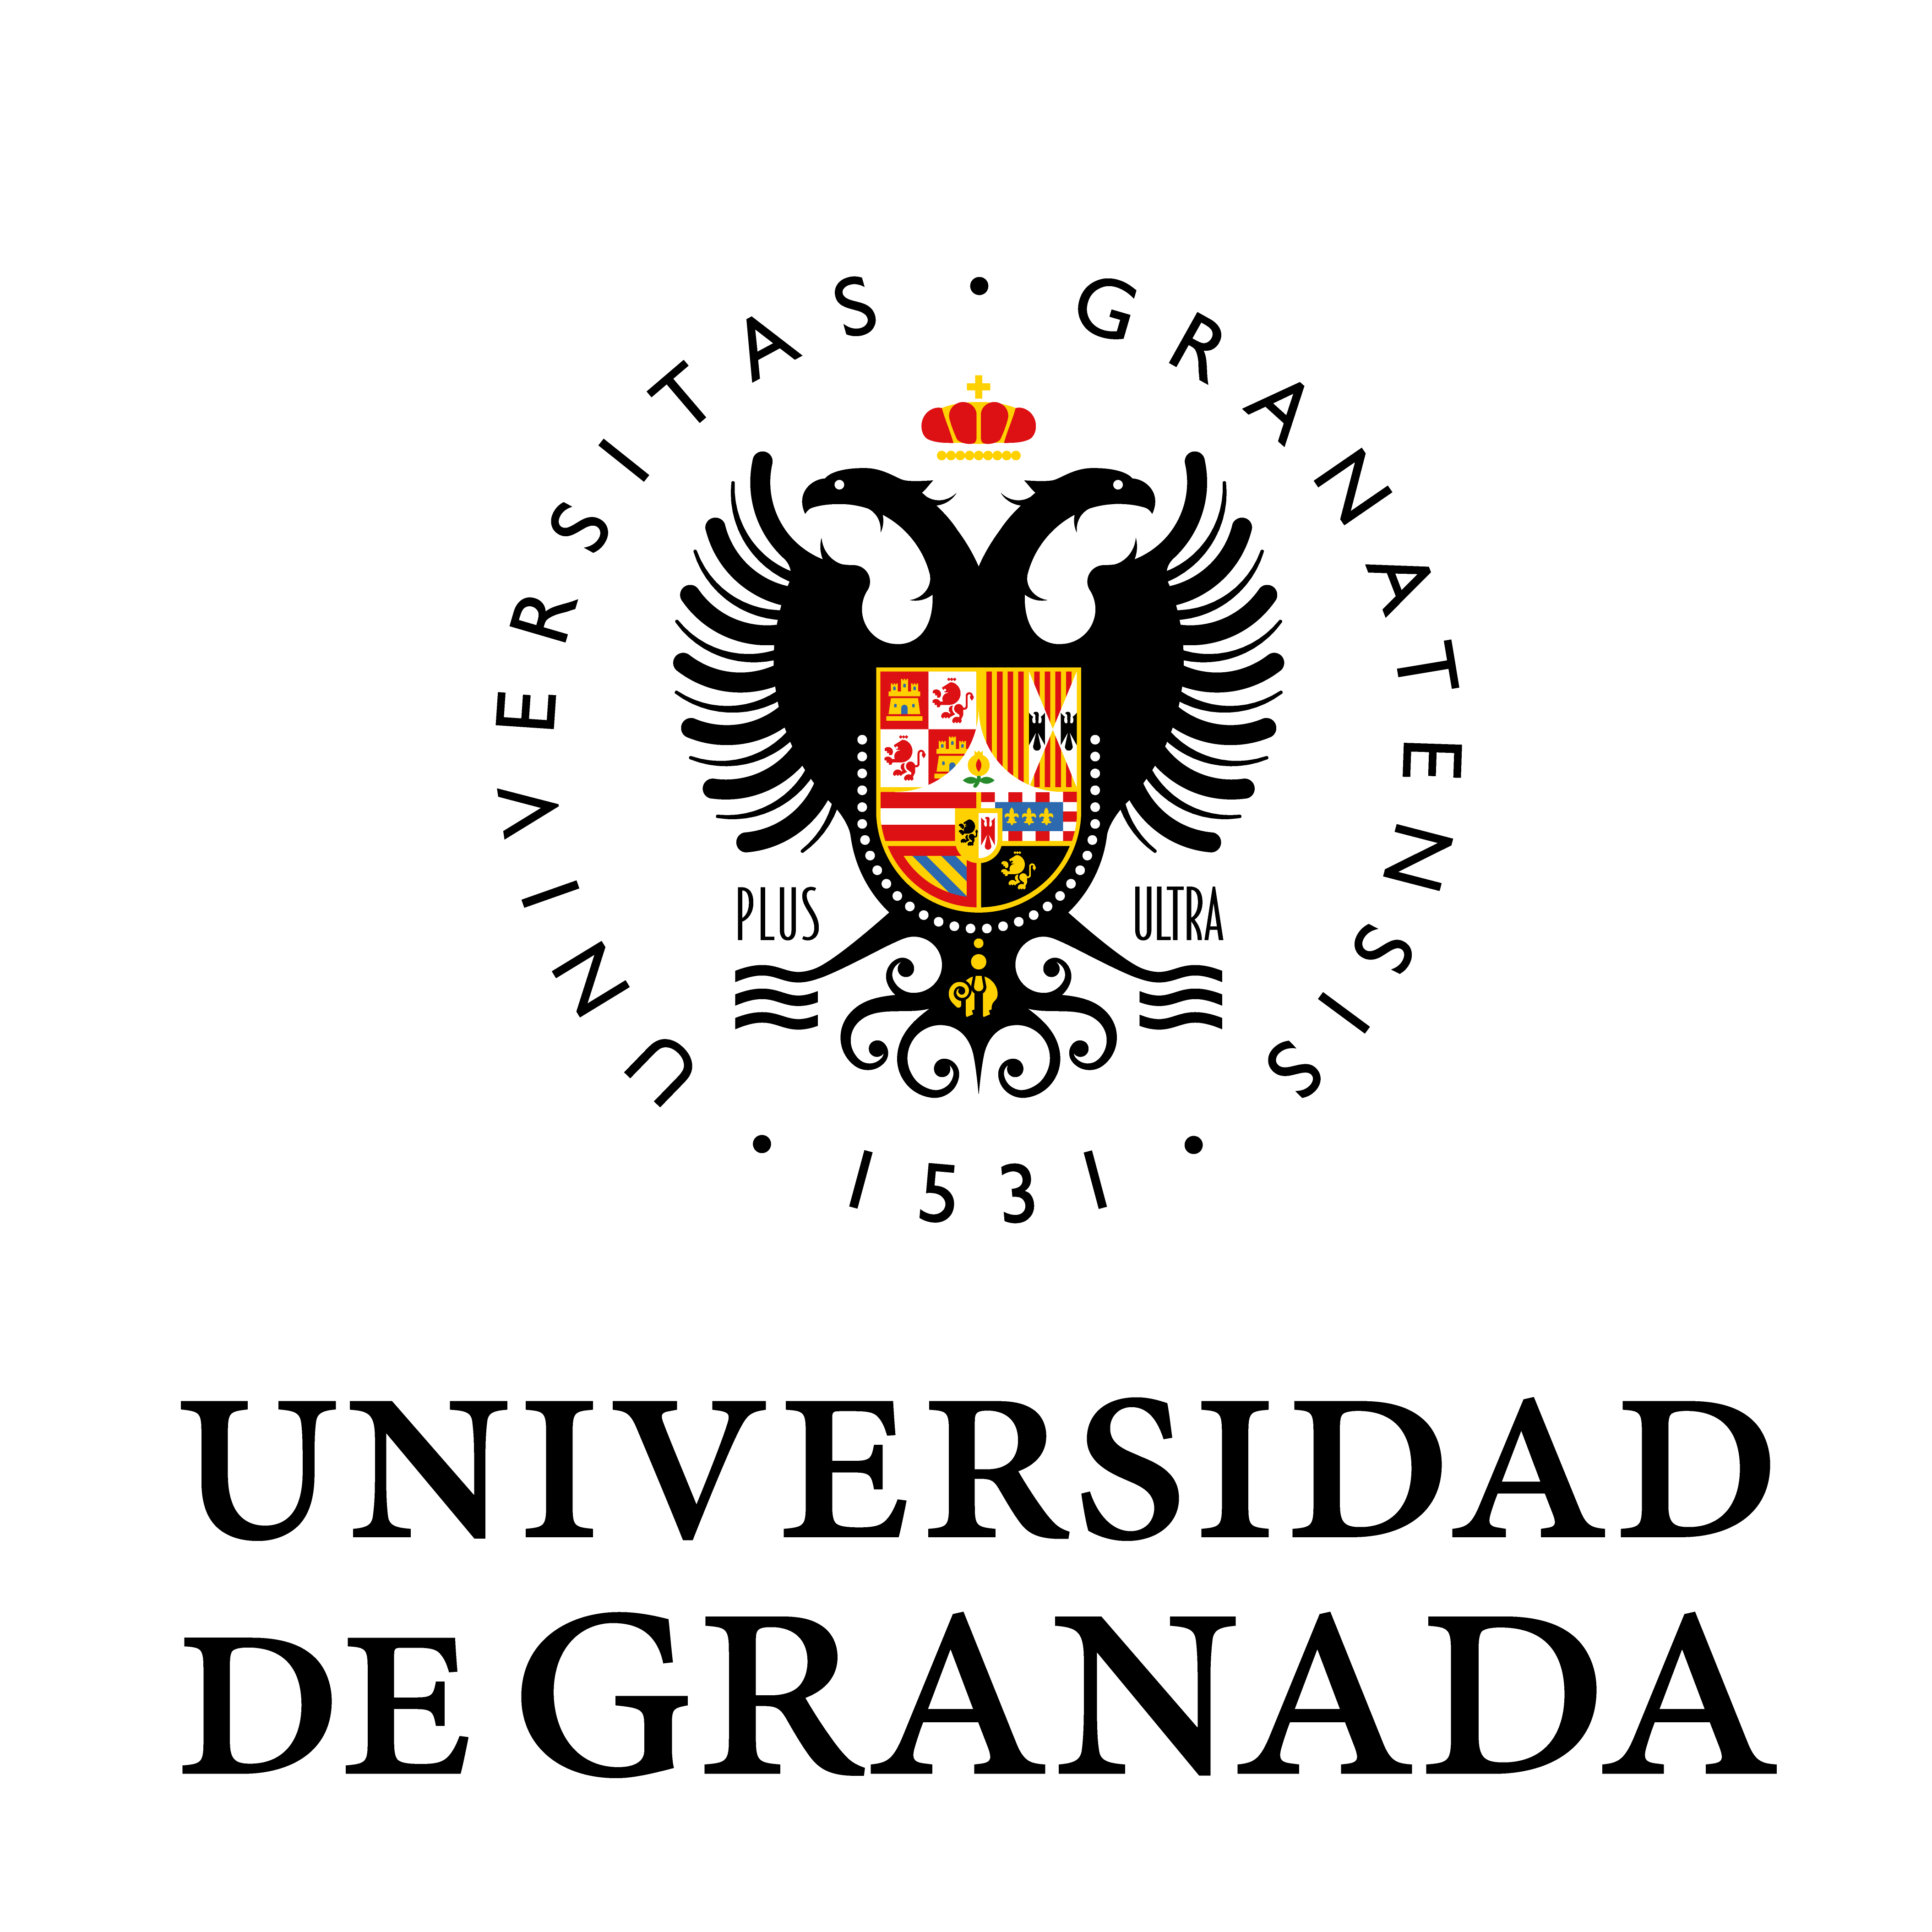
\includegraphics[width=6cm]{gfx/UGRlogo.png} \\ \medskip

        %\mySubtitle \\ \medskip
        %\myDegree \\
        %\myDepartment \\
        %\myFaculty \\
        %\myUni \\ \bigskip

        \myTime\

        \vfill

        \myProf, \myOtherProf \\
        %\myFaculty \\
        \myUni \\ \bigskip


    \end{center}
%  \end{addmargin}

\end{titlepage}

\thispagestyle{empty}

\hfill

\vfill

\textbf{Licencia} \ccbysa

Este trabajo está bajo una licencia \hyperlink{https://creativecommons.org/licenses/by-sa/4.0/legalcode}{Creative Commons Attribution - ShareAlike 4.0 International License}.

Con esta licencia, puedes:
\begin{itemize}
	\item  Compartir, copiar, y redistribuir el contenido.
	\item  Modificar el material de cualquier forma, incluso con propósito comercial.
\end{itemize}

Con las siguientes obligaciones:
\begin{itemize}
	\item[\ccAttribution] Dar el crédito apropiado, aportando un enlace a la licencia, e indicar los cambios realizados. 
	\item[\ccShareAlike] Cualquier copia, o modificación debe ser distribuida con la misma licencia que el original.
	\item[] No aplicar medidas de carácter legal o tecnológico que impidan a otros hacer aquello que la licencia permita.
\end{itemize}
\clearpage

\cleardoublepage\include{FrontBackmatter/Dedication}
%\cleardoublepage\include{FrontBackmatter/Foreword}
\cleardoublepage%*******************************************************
% Abstract
%*******************************************************
\begingroup
\let\clearpage\relax
\let\cleardoublepage\relax
\let\cleardoublepage\relax

\pdfbookmark[1]{Abstract}{Abstract}
\chapter*{Abstract}

In this work, we define the basics of singular homology theory, starting with the necessary geometric constructions
and the definition of the singular homology groups. Following the definitions and a proof of homotopy invariance,
we prove the baricentric subdivision theorem, the central result of this work, that leads us inmediatly to the
Mayer-Vietoris sequence. This and other results are applied to obtain the homology groups of the spheres and a number
of classical theorems, including the Brower fixed-point theorem and the Jordan-Brower separation theorem.

On the second part, we introduce the maximum clique problem, a well studied combinatorial optimization problem, known
to be NP-hard. Due to this, the use of metaheuristics is necessary to solve it in reasonable time. Several heuristics
are considered, explained in detail and applied to DIMACS instances. We discuss their behaviour and compare them,
showing which of the proposed algorithms can yield satisfactory results.


\paragraph{keywords} Homology theory, Homotopy invariance, Baricentric subdivision theorem, Mayer-Vietoris sequence,
Maximum clique, Combinatorial optimization problem, Metaheuristics, NP-hard, DIMACS.

\vfill

\endgroup

\vfill

\cleardoublepage\include{FrontBackmatter/Publications}
\cleardoublepage\include{FrontBackmatter/Acknowledgments}
\pagestyle{scrheadings}
\cleardoublepage%*******************************************************
% Table of Contents
%*******************************************************
%\phantomsection
\refstepcounter{dummy}
\pdfbookmark[1]{\contentsname}{tableofcontents}
\setcounter{tocdepth}{2} % <-- 2 includes up to subsections in the ToC
\setcounter{secnumdepth}{3} % <-- 3 numbers up to subsubsections
\manualmark
\markboth{\spacedlowsmallcaps{\contentsname}}{\spacedlowsmallcaps{\contentsname}}
\tableofcontents
\automark[section]{chapter}
\renewcommand{\chaptermark}[1]{\markboth{\spacedlowsmallcaps{#1}}{\spacedlowsmallcaps{#1}}}
\renewcommand{\sectionmark}[1]{\markright{\thesection\enspace\spacedlowsmallcaps{#1}}}
%*******************************************************
% List of Figures and of the Tables
%*******************************************************
\clearpage

\begingroup
    \let\clearpage\relax
    \let\cleardoublepage\relax
    \let\cleardoublepage\relax
    %*******************************************************
    % List of Figures
    %*******************************************************
    %\phantomsection
    \refstepcounter{dummy}
    %\addcontentsline{toc}{chapter}{\listfigurename}
    \pdfbookmark[1]{\listfigurename}{lof}
    \listoffigures

    \vspace{8ex}

    %*******************************************************
    % List of Tables
    %*******************************************************
    %\phantomsection
    \refstepcounter{dummy}
    %\addcontentsline{toc}{chapter}{\listtablename}
    \pdfbookmark[1]{\listtablename}{lot}
    \listoftables

    \vspace{8ex}
%   \newpage

    %*******************************************************
    % List of Listings
    %*******************************************************
      %\phantomsection
    %\refstepcounter{dummy}
    %\addcontentsline{toc}{chapter}{\lstlistlistingname}
    %\pdfbookmark[1]{\lstlistlistingname}{lol}
    %\lstlistoflistings

    %\vspace{8ex}

    %*******************************************************
    % Acronyms
    %*******************************************************
    %\phantomsection
    %\refstepcounter{dummy}
    %\pdfbookmark[1]{Acronyms}{acronyms}
    %\markboth{\spacedlowsmallcaps{Acronyms}}{\spacedlowsmallcaps{Acronyms}}
    %\chapter*{Acronyms}
    %\begin{acronym}[UMLX]
    %    \acro{DRY}{Don't Repeat Yourself}
    %    \acro{API}{Application Programming Interface}
    %    \acro{UML}{Unified Modeling Language}
    %\end{acronym}                     
\endgroup

%********************************************************************
% Mainmatter
%*******************************************************
\cleardoublepage\pagenumbering{arabic}
%\setcounter{page}{90}
% use \cleardoublepage here to avoid problems with pdfbookmark
\cleardoublepage

% Parte 1: Matemáticas.
% Homología Singular


\part{Homología Singular}
%************************************************
\chapter{Introducción}\label{ch:introduccion}
%************************************************

\section{Definiciones iniciales}

En este capítulo, introduciremos la \textbf{homología singular} de un espacio topológico. Comenzaremos con
un conjunto de definiciones iniciales, introduciendo la noción de \textbf{símplice singular}. Con ellos,
construiremos un conjunto al que dotaremos de estructura algebraica, y sobre el que definiremos una aplicación
que, gracias a sus propiedades, nos permitirá definir la homología singular del espacio. Seguidamente,
demostraremos algunos resultados sencillos sobre ciertos espacios topológicos, continuando con la invarianza
homotópica de la homología. Concluiremos el capítulo definiendo la homología sobre pares topológicos, y
viendo como se trasladan los resultados demostrados con anterioridad.

\begin{definition}
Un \textbf{p-símplice} $s_p$ es la envolvente conexa de $p+1$ puntos afínmente independientes en $\mathbb{R}^p$,
a los que llamaremos vértices, $\{x_0, \dots, x_n\}$, esto es
\[ s_p = \{\lambda_0 x_0 + \dots + \lambda_p x_p \mid \lambda_0 + \dots + \lambda_p = 1, \lambda_i \geq 0 \hspace{0.2em} \forall i \} \]
\end{definition}
% \underbrace{\smash{1}}_{i}
Cuando los vértices son $x_i = (0, \dots, 1, \dots, 0)$, con el $1$ en la posición $i$-ésima, le llamaremos el p-símplice \underline{standard},
y lo notaremos por $\sigma_p$.

Podemos establecer un homeomorfismo $h \colon \sigma_p \to s_p$ por
\[ h(t_0, \dots, t_p) = \sum\limits_{i = 0}^p t_i x_i \]

\begin{definition}
Sea $\X$ un espacio topológico. Un \textbf{p-símplice singular} en $\mathbb{X}$ es una aplicación continua $\phi \colon \sigma_p \to \X$ para $p \geq 0$.
\end{definition}

Representaremos el conjunto de p-símplices singulares de $\mathbb{X}$ como
\[F_p(\mathbb{X}) = \{\phi \colon \sigma_p \to \mathbb{X} \mid \phi \text{ es p-símplice singular}\}\]
Es claro que $\mathbb{F}_0(\mathbb{X}) = \mathbb{X}$. Además, $F_1(\mathbb{X})$ son los arcos en $\X$, identificables por
$\mathbb \mathcal{C}([0,1], \X)$.

Si tenemos una aplicación continua entre espacios topológicos $f \colon \X \to \Y$, podemos definir
\[f_{\#} \colon \FX{p} \to \FY{p}  \quad \text{ por }  \quad f_{\#} = f \circ \phi \colon \sigma_p \to Y \]
que es una aplicación entre los p-símplices singulares de ambos espacios.

Se verifica trivialmente que $I_\# = Id$, puesto que $I_\#(\phi) = I \circ \phi = \phi$.
Además, se tiene que $(g \circ f)_\# = g_\# \circ f_\#$.

\begin{definition}
  Sea $p \geq 1$, $0 \leq i < p$. Definimos $F_p^i$ como la aplicación de un $(p-1)$-símplice a un p-símplice de la siguiente forma:
  \begin{align*}
    F_p^i \colon \sigma_{p-1} &\to \sigma_p\\
    (t_0, \dots, t_{p-1}) &\mapsto (t_0, \dots, t_{i-1}, 0, t_i, \dots, t_{p-1})
  \end{align*}

  Podemos definir una nueva aplicación a partir de esta, a la que llamaremos \textbf{i-esima cara}:
  \begin{align*}
    \partial_i \colon \FX{p} &\to \FX{p-1}\\
    \partial_i(\phi) &= \phi \circ F_p^i
  \end{align*}
\end{definition}

Vamos a probar un resultado sobre la aplicación que acabamos de definir.

\begin{lemma}
  Se verifica que $F_p^i \circ F_{p-1}^j = F_p^j \circ F_{p-1}^{i-1} \quad \forall p \geq 2$, $\forall i, j \colon 0 \leq j < i \leq p$.
\end{lemma}

\begin{proof}
Lo comprobamos realizando los cálculos pertinentes
  \begin{align*}
    &F_p^i \circ F_{p-1}^j (t_0, \dots, t_{p-2}) = F_p^i (t_0, \dots, t_{j-1}, 0, t_j, \dots, t_{p-2}) \\
    &= (t_0, \dots, t_{j-1}, 0, t_j, \dots, t_{i-2}, 0, t_{i-1}, \dots, t_{p-2}) \\
    &= F_p^j (t_0, \dots, t_{i-2}, 0, t_{i-1}, \dots, t_{p-2}) = F_p^j \circ F_{p-1}^{i-1} (t_0, \dots, t_{p-2}).
  \end{align*}
\end{proof}

Se deduce directamente este corolario:

\begin{corollary}
  Para $p \geq 2, 0 \leq j < i \leq p$, se verifica $\partial_j \circ \partial_i = \partial_{i-1} \circ \partial_j$.
\end{corollary}

Debido a que $\FX{p}$ no está dotado de estructura algebraica, es posible realizar la siguiente construcción:

\begin{definition}
  Si $\X$ es un espacio topológico, y $p \geq 0$, se define el \textbf{grupo de p-cadenas singulares} de $\X$
  como el grupo abeliano libre generado por $\FX{p}$
  \[ S_p(\X) = \{\sum_{\phi \in \FX{p}} n_\phi \cdot \phi  \mid n_\phi \in \Z \text{, todos cero salvo un número finito} \}\]

  Podemos definir un operador \textbf{borde} $\partial$ con las aplicaciones cara $\partial_i$ de la siguiente forma:
  \begin{align*}
    \partial \colon S_p(\X) &\to S_{p-1}(\X)\\
    \partial(\phi) &= \sum_{i = 0}^p (-1)^i \partial_i(\phi)  \hspace{1cm} (p \geq 1)
  \end{align*}
  considerando $\partial_i$ como una extensión de la aplicación cara a un homomorfismo:
  \[\partial_i(\sum_{\phi \in F_p} n_\phi \cdot \phi) = \sum_{\phi \in F_p} n_\phi \cdot \partial_i(\phi) \]
\end{definition}

Por conveniencia, consideraremos $\partial(S_0(\X)) = S_{-1}(\X) = \{0\}$.

% Motivar (mejor) el resultado siguiente?

Veamos un resultado importante sobre la aplicación borde que acabamos de definir.

\begin{proposition}
  $\partial \circ \partial \colon \SX{n} \to \SX{n-2}$ es el homomorfismo cero.
\end{proposition}

Geométricamente, este resultado nos dice que el borde de una $p$-cadena es una $(p-1)$-cadena sin
borde. Esta propiedad nos permitirá definir los grupos de homología singular.

\begin{proof}
  Consideramos $S_p(\X) \xrightarrow{\partial} S_{p-1}(\X) \xrightarrow{\partial} S_{p-2}(\X)$. \\
  Es claro que si $p = 0, 1$, la cuestión es trivial, pues $S_{-1} = \{0\}$. Tomaremos $p > 1$.

  Sea $\phi \in \FX{p}$.
  \begin{align*}
    \partial^2(\phi) &= \partial(\sum_{i = 0}^p (-1)^i \partial_i(\phi)) = \sum_{i = 0}^p (-1)^i \partial(\partial_i(\phi)) \\
                     &= \sum_{i = 0}^p (-1)^i \sum_{j = 0}^{p-1} (-1)^j \partial_j \partial_i(\phi) \\
                     &= \sum_{0 \leq j < i \leq p} (-1)^{i + j} \partial_j \partial_i(\phi)
                        + \sum_{0 \leq i \leq j \leq p-1} (-1)^{i + j} \partial_j \partial_i(\phi) \\
                     &= \sum_{0 \leq j < i \leq p} (-1)^{i + j} \partial_{i-1} \partial_j(\phi)
                        + \sum_{0 \leq i \leq j \leq p-1} (-1)^{i + j} \partial_j \partial_i(\phi) \\
                     &= \sum_{0 \leq j \leq i-1 \leq p} (-1)^{i + j} \partial_{i-1} \partial_j(\phi)
                        + \sum_{0 \leq i \leq j \leq p-1} (-1)^{i + j} \partial_j \partial_i(\phi) = 0\\
                     &\text{pues son iguales salvo el signo.}
  \end{align*}
\end{proof}

Hasta ahora, hemos tomado un espacio topológico $\X$ y le hemos asignado un conjunto de p-símplices singulares $\FX{p}$, del que
hemos tomado un $\Z$-módulo, obteniendo el grupo abeliano libre de p-cadenas singulares, $S_p(\X)$. Sobre él, hemos definido un
operador borde $\partial$, que verifica $\partial^2 = 0$. A la familia $\{S_p(\X), \partial\}_{p \geq 0}$ se le llama el complejo de cadenas
singular asociado a $\X$.

Representaremos también por $f_\# \colon S_p(\X) \to S_p(\Y)$ a la composición entre
$f \colon \X \to \Y$, continua, y $\phi \in S_p(\X)$.
\[ f_\#(\sum_\phi n_\phi \cdot \phi) = \sum_\phi n_\phi \cdot (f \circ \phi) \]

Vamos a ver que esta aplicación conmuta con el borde, es decir, $f_\# \circ \partial = \partial \circ f_\#$. Esto hace conmutativo el siguiente diagrama:
\[
  \begin{tikzcd}
    \dots S_{p+1}(\X) \arrow{r}{\partial} \arrow{d}{f_\#} & S_p(\X) \arrow{r}{\partial} \arrow{d}{f_\#} & S_{p-1}(\X) \arrow{d}{f_\#} \dots \\
    \dots S_{p+1}(\Y) \arrow{r}{\partial}                 & S_p(\Y) \arrow{r}{\partial}                 & S_{p-1}(\Y) \dots
  \end{tikzcd}
\]

Su demostración es casi inmediata, pues se tiene que \[ f_\# \circ \partial_i(\phi) = f_\#(\phi \circ F_p^i) = f \circ \phi \circ F_p^i
                                             = \partial_i(f \circ \phi) = \partial_i \circ f_\#(\phi) \]

El resultado obtenido implica, por la definición de $\partial$, que $\partial f_\# = f_\# \partial$. De hecho, es más fuerte, pues vemos
como las aplicaciones cara conmutan una a una con el homomorfismo $f_\#$.

A esta aplicación entre complejos de cadenas se le llama en álgebra una aplicación de cadenas. Nos referiremos a ella como la aplicación de cadenas
inducida por la aplicación continua f.

\begin{definition}
  Diremos que $c \in S_p(\X)$ es un \textbf{p-ciclo} si $\partial(c) = 0$. \\
  Diremos que $c \in S_p(\X)$ es un \textbf{p-borde} si existe $d \in S_{p+1}(\X) \text{ tal que } \partial(d) = c$.
\end{definition}

% ¿Indentar los conjuntos?

Representaremos por: \\
$Z_p(\X) = \{c \in S_p(\X) \mid \text{ c es un p-ciclo}\}$ \\
$B_p(\X) = \{c \in S_p(\X) \mid \text{ c es un p-borde}\} $

Se verifica que: \\
$Z_p(\X) = \Ker (\partial \colon S_p(\X) \to S_{p-1}(\X)) $ \\
$B_p(\X) = \Img (\partial \colon S_{p+1}(\X) \to S_p(\X)) $

Ambos son subgrupos de $S_p(\X)$, llamados grupos de los ciclos y los bordes, respectivamente. Como hemos visto que $\partial^2 = 0$, se deduce
inmediatamente que $B_p(\X) \subseteq Z_p(\X) \hspace{0.2em}\forall p \geq 0$, luego se puede construir el grupo cociente.
\begin{equation*}
  H_p(\X) = \ddfrac{Z_p(\X)}{B_p(\X)}
\end{equation*}
al que llamaremos el \textbf{\underline{\smash{p-ésimo grupo de homología singular}}}, el cual es un grupo abeliano.

\begin{remark}
  Nótese que $Z_0(\X) = S_0(\X)$, pues $\partial(S_0(X)) = 0$.
\end{remark}

A los elementos de $H_p(\X)$ los notaremos $[c]$, con $\partial(c) = 0$, esto es, $c \in Z_p(\X)$, y los llamaremos clases de homología.

La motivación geométrica para la construcción de los grupos de homología singular se basa en querer
estudiar los ciclos en espacios topológicos. Como este conjunto tiene un tamaño demasiado grande para
poder estudiarlo de forma efectiva, restringimos nuestra atención a las clases de equivalencia, haciendo
que dos ciclos sean equivalentes si su diferencia es el borde de una cadena en una dimensión superior.

Tomemos nuevamente una función continua $f \colon \X \to \Y$, y definamos
\[ f_* \colon H_p(\X) \to H_p(\Y) \quad f_*([c]) = [f_\#(c)]  \]

Comprobemos que está bien definida, esto es, que no depende del representante que se elija.

Sean $[c_1] = [c_2]$, lo que implica $c_1 - c_2 \in B_p(\X)$. Por tanto, existe $d \in S_{p+1}(\X)$ tal que $\partial(d) = c_1 - c_2$.
Así, $f_\#(c_1) - f_\#(c_2) = f_\#(c_1 - c_2) = f_\#(\partial(d)) = \partial(f_\#(d))$ \\
Como $f_\#(d) \in S_{p+1}(\Y)$, se tiene $[f_\#(c_1)] = [f_\#(c_2)]$

Además, $\partial(f_\#(c)) = f_\#(\partial(c)) = 0$, por lo que $f_\#(c)$ es un ciclo en $\Y$. Con esto hemos visto que $f_*$ está bien definida,
y es un homomorfismo, al serlo $f_\#$, al que llamaremos homomorfismo inducido por f en la homología.

De las propiedades de $f_\#$ obtenemos directamente que:
\begin{itemize}
  \item $(g \circ f)_* = g_* \circ f_*$
  \item $I_* = Id$
\end{itemize}

Así, hemos construído un funtor covariante de la categoría de espacios topológico en la categoría de grupos abelianos,
el funtor de la homología singular.
\[  \begin{tikzcd}
  \X \arrow{r} \arrow{d}{f} & [5em] H_p(\X) \arrow{d}{f_*} \\
  \Y \arrow{r}  & H_p(\Y)
\end{tikzcd} \]

Si $\X$ e $\Y$ son homeomorfos, el homomorfismo que induce dicho homeomorfismo en la homología es un isomorfismo de grupos de homología, pues
basta considerar el inverso del homeomorfismo para construir el inverso del homomorfismo inducido.

\section{Homología de un punto}

Vamos a calcular los grupos de homología singular de los puntos, sin más que ver como se comporta la función borde
en ellos y utilizando la definición de los grupos de ciclos y bordes como núcleo e imagen de dicha aplicación.

Sea $\X$ un espacio topológico formado por un punto, $\X = \{x\}$.
$\FX{p} = \{ \phi \colon \sigma_p \to \{x\} \} = \{\phi_p\}$ donde $\phi_p$ es la función constante.

$S_p({\{x\}})$ son grupos abelianos libres con $\phi_p$ como generador. Además, $\partial \colon \SX{p} \to \SX{p-1}$ verifica:
\[\partial(\phi_p) = \sum_{i = 0}^p (-1)^i \partial_i(\phi_p) =  \sum_{i = 0}^p (-1)^i \phi_{p-1} = \begin{cases}
                                                                                                            0 & p \text{ es impar} \\
                                                                                                            \phi_{p-1} & p \text{ es par}
                                                                                                    \end{cases}   \]

Así, si p es impar, $S_{p+1}(\{x\}) \to S_p(\{x\}) \xrightarrow{0} S_{p-1}(\{x\})$ y $Z_p(\{x\}) = B_p(\{x\}) = S_p(\{x\})$, luego
$H_p(\{x\}) = 0$.

Si p es par, con $p > 0$, $Z_p(\{x\}) = B_p(\{x\}) = 0$, y $H_p(\{x\}) = 0$.

Por último, si $ p = 0, H_0(\{x\}) = \ddfrac{S_0(\{x\})}{B_0(\{x\})} = S_0(\{x\}) \cong \mathbb Z$.

Así, $H_p(\{x\}) = 0 \hspace{1em} \forall p \geq 1, \hspace{1em} H_0(\{x\}) \cong \mathbb Z$.

\section{El grupo $H_0(\X)$ y la arcoconexión}

En esta sección vamos a estudiar algunas de las propiedades de los grupos de homología singular, asumiendo que el espacio
sobre el que trabajamos es arcoconexo.

\begin{proposition}
  Sea $\X$ un espacio topológico arcoconexo. Entonces $H_0(\X) \cong \mathbb Z$.
\end{proposition}

\begin{proof}
  Consideramos $\SX{1} \xrightarrow{\partial} \SX{0} \to \{0\}$. Tomamos $H_0(\X)$.

  $H_0(\X) = \ddfrac{Z_0(\X)}{B_0(\X)} = \ddfrac{S_0(\X)}{\Img \partial}$

  Sea $\epsilon \colon S_0(\X) \to \Z$ definido por \[\epsilon(\sum\limits_{\phi} n_\phi \phi) = \epsilon(\sum\limits_{x} n_x \cdot x) = \sum\limits_{x} n_x \]
  suma finita, por cómo definimos $S_0$.

  Se verifica que $\epsilon$ es un epimorfismo de grupos, pues podemos definir el conveniente elemento de $S_0(\X)$ para obtener
  cualquer entero. Calculamos el núcleo de la aplicación:
  \[ \epsilon \circ \partial(\phi_1) = \epsilon(\sum_{i=0}^1 \partial_i(\phi_i)) = 1 - 1 = 0\]  Así, $\Img \partial \subseteq \Ker \epsilon$.

  Sea ahora $\sum n_x \cdot x \in \Ker \epsilon$, esto es, $\sum n_x = 0$. \\
  $\sum n_x \cdot x = n_1 x_1 + \dots + n_k x_k$ con $\sum\limits_{i=1}^k = 0, x_i \in \X$. \\
  Sean $\phi^i \colon \sigma_1 \to \X$ arcos tales que $\phi^i(e_1) = x_i, \phi^i(e_0) = x$,
  donde $e_1, e_0$ representan los vértices de $\sigma_1$ y $x \in \X$ es un punto fijo.
  Es posible hacer esta construcción gracias a la arcoconexión de $\X$. De esta forma:
  \begin{align*}
    &\sum_i n_i \phi^i \in \SX{1}, \text{ y se tiene} \\
    &\partial(\sum_i n_i \phi^i) = \sum_i n_i \partial(\phi^i) = \sum_i n_i(x_i - x) = (\sum_i n_i x_i) - (\sum_i n_i) x = \sum_i n_i x_i
  \end{align*}
  De aquí se deduce que $\Ker \epsilon \subseteq \Img \partial$, y por tanto tenemos la igualdad.

  Finalmente como $\Ker \epsilon = \Img \partial$, $H_0(\X) = \ddfrac{S_0(\X)}{\Ker \epsilon} \cong \Z$, al ser $\epsilon$ epimorfismo.
\end{proof}

\begin{proposition}
  Sea $\X$ un espacio topológico, $\X = \bigcup\limits_{\alpha \in A} \X_\alpha$ su descomposición en componentes arcoconexas. Entonces se verifican:
  \begin{itemize}
    \item[a)] $\forall \alpha \in A$, la función $i_{\alpha*} \colon H_p(\X_\alpha) \to H_p(\X)$ es un monomorfismo, donde la aplicación
              $i_\alpha \colon \X_\alpha \to \X$ representa la inclusión.
    \item[b)] $H_p(\X) = \bigoplus\limits_{\alpha \in A} i_{\alpha*}(H_p(\X_\alpha)) \hspace{0.5em} \forall p \geq 0$. En particular, por la inyectividad de $i_{\alpha*}$,
              \[ H_p(\X) \cong \bigoplus_{\alpha \in A} H_p(\X_\alpha) \]
  \end{itemize}
\end{proposition}

\begin{proof}
  Sea $\phi \colon \sigma_p \to \X$ un p-símplice singular. Como $\sigma_p$ es convexo y $\phi$ es continua, $\phi(\sigma_p) \subseteq \X_\alpha$, para algún
  $\alpha \in A$, por lo que $\phi = i_{\alpha*}(\phi)$ para dicho $\alpha$. \\
  Si $c = \sum n_\phi \cdot \phi$ es una p-cadena, poniendo cada $\phi$ de la forma anterior y agrupando por componentes conexas:
  \begin{equation}
    c = \sum\limits_{\alpha \in A} i_{\alpha*}(c_\alpha), \quad c_\alpha \in S_p(\X_\alpha)  \tag{*}
  \end{equation}

  Sea $[c]_\alpha \in H_p(\X_\alpha)$, y supongamos que $i_{\alpha*}[c]_\alpha = 0$ en $\H_p(\X)$. En ese caso, $[i_{\alpha*}(c)] = 0$ en $H_p(\X)$,
  luego existe $d \in \SX{p+1}$ tal que $i_{\alpha\#}(c) = \partial(d)$, y además:
  \[\partial(d) = \sum\limits_{\beta \in A} i_{\beta\#}(\partial(d_\beta)) = i_{\alpha\#}(c) \]
  por lo que se tiene $c = \partial(d_\alpha), \partial(d_\beta) = 0 \hspace{0.5em} \forall \beta \neq \alpha$. Así, $[c]_\alpha = 0$ y $i_{\alpha*}$ es un monomorfismo.
  Esto prueba a).

  Observamos que la suma en (*) es finita, pues si no, habría un número no finito de generadores en la expresión de c. Así:
  \[  [c] = \sum\limits_{\alpha \in A} [i_{\alpha\#}(c_\alpha)] =  \sum\limits_{\alpha \in A} i_{\alpha*}([c_\alpha]_\alpha)\]

  Como $\partial(c) = 0 \iff \partial(c_\alpha) = 0 \hspace{0.5em} \forall \alpha \in A$, se obtiene directamente b), como consecuencia de a).
\end{proof}

En particular, para $H_0(\X)$, por el resultado anterior, se tiene que $H_0(\X)$ es el grupo abeliano libre con tantos generadores como
componentes arcoconexas tenga $\X$.

\section{Invarianza homotópica de la homología singular}

En esta sección demostraremos la invarianza de los grupos de homología singular en espacios homotópicamente equivalentes, viendo antes como
dos aplicaciones homotópicas inducen el mismo homomorfismo en la homología.

Vamos a comenzar demostrando el llamado Lema de Poincaré.

\begin{lemma}[Lema de Poincaré]
  Sea $\X \subseteq \R^n$ estrellado desde algún punto. Entonces:
  \[ H_p(\X) = \begin{cases}  \Z & \text{ si } p = 0 \\
                              0  & \text{ si } p \neq 0
                            \end{cases} \]
\end{lemma}

\begin{proof}
  El caso $p = 0$ está claro, pues un conjunto estrellado es, en particular, arcoconexo, por lo que solo hemos de aplicar el resultado ya demostrado.
  Suponemos $p > 0$.

  Para demostrarlo, vamos a construir un homomorfismo $ T: \SX{p} \to \SX{p+1}$ tal que $ T \partial + \partial  T = Id_{\SX{p}}$ para $p > 0$.

  De darse la situación anterior, si $[c] \in H_p(\X), c \in Z_p(\X)$, se tiene $\partial(c) = 0$ y $c \in S_p(\X)$.
  En consecuencia, $c = (\partial  T +  T \partial)(c)  = \partial( T(c))$ con $ T(c) \in \SX{p+1}$.
  Por tanto, $c$ es un borde, luego $[c] = 0$, y eso implica que $H_p(\X) = 0 \quad \forall p > 0$.

  Definamos $T$: \\
  Sean $x_0 \in \X$ un punto de estrella, $\phi \colon \sigma_p \to \X$ un p-símplice singular. Tomemos $T(\phi) \colon \sigma_{p+1} \to \X$ dado por:
  \[ T(\phi)(t_0,\dots,t_{p+1}) = \begin{cases} x_0 & \text{ si } t_0 = 1 \\
                                                (1-t_0)\phi(\frac{t_1}{1-t_0},\dots,\frac{t_{p+1}}{1-t_0}) + t_0 x_0 & \text{ si } t_0 < 1
                                  \end{cases} \]
  Como $\X$ es estrellado, $\Img(T(\phi)) \subseteq \X$.

  Veamos que $T(\phi)$ es continuo. \\
  La continuidad está clara para $t_0 < 1$, por lo que la vemos para $t_0 = 1$. Se verifica que:
  \begin{align*}
    &|T(\phi)(t_0,\dots,t_{p+1}) - x_0| = |t_0 x_0 + (1-t_0)\phi(\frac{t_1}{1-t_0},\dots,\frac{t_{p+1}}{1-t_0}) - x_0| \\
    &= (1-t_0)|\phi(\frac{t_1}{1-t_0},\dots,\frac{t_{p+1}}{1-t_0}) - x_0| \leq (1-t_0)(c + |x_0|) \\
    & \text{ pues $\phi$ está acotada.}
  \end{align*}

  Así, $\lim\limits_{t_0 \to 1} T(\phi) = x_0$.

  Queda claro que $\partial_0(T(\phi)) = \phi$. Si seguimos llamando $T$ al homomorfismo extensión de $T$ a $\SX{p}$, tenemos construído
  \[  T \colon \SX{p} \to \SX{p+1} \hspace{0.5em} \text{tal que } \partial_0 \circ  T = I. \]
  Si $p = 0 \implies i = 1$ y $\partial_1( T(\phi)) = x_0$.

  Si $1 \leq i \leq p+1$, entonces:
  \begin{align*}
    &\partial_i( T(\phi))=(t_0,\dots,t_p)) =  T(\phi)(t_0, \dots, t_{i-1} \circ t_i, \dots, t_p) \\
    &= (1-t_0)\phi(\frac{t_1}{1-t_0}, \dots, \frac{t_{i-1}}{1-t_0}, \dots, \frac{t_p}{1-t_0}) + t_0 x_0 \\
    &= (1-t_0)\partial_{i-1}(\frac{t_1}{1-t_0}, \dots, \frac{t_p}{1-t_0}) + t_0 x_0 = T(\partial_{i-1} \phi)(t_0, \dots, t_p)
  \end{align*}
  Como consecuencia:
  \begin{align*}
    \partial( T(\phi)) &= \sum\limits_{i = 1}^{p+1} (-1)^i \partial_i  T(\phi) = \phi + \sum\limits_{i = 1}^{p+1} (-1)^i  T \partial_{i-1}(\phi) \\
    &= \phi - \sum\limits_{j = 0}^p (-1)^j  T \partial_j(\phi) = \phi -  T \partial(\phi)
  \end{align*}

  De donde se obtiene directamente que $\partial  T +  T \partial = Id$.
\end{proof}

\begin{theorem}[Invarianza homotópica de la homología singular]
  Sean $\X, \Y$ espacios topológicos y $f, g \colon \X \to \Y$ aplicaciones continuas. Si $f$ es homotópica a $g$,
  entonces $f_* = g_* \colon H_p(\X) \to H_p(\Y) \hspace{0.5em} \forall p \geq 0$.
\end{theorem}

\begin{proof}
  Supongamos que $\forall p \geq 0$ podemos definir homomorfismos \[T: \SX{p} \to \SY{p+1} \] tales que $T\partial + \partial T = f_\# - g_\#$,
  esto es, $f$ y $g$ son homotópicas como aplicaciones de cadenas. Entonces, $\forall [c] \in H_p(\X)$ se tiene:
  \[ (f_* - g_*)([c]) = [f_\#(c) - g_\#(c)] = [(T\partial + \partial T)(c)] = [\partial(T(c))] = 0\]
  de donde se deduce $f_* = g_*$.

  Veamos la definición de dicho $T$.

  Sea $H \colon \X \times I \to \Y$ la homotopía entre f y g, esto es,
  \[H(x, 0) = f(x), \quad H(x, 1) = g(x)\]
  donde $I$ representa el intervalo $[0, 1]$.

  Sean $i_0, i_1 \colon \X \to \X \times I$ dados por $i_0(x) = (x, 0), i_1(x) = (x, 1)$. Es claro que $f = H \circ i_0, g = H \circ i_1$, de donde
  se tiene \[ f_\# - g_\# = H_\# \circ i_{0\#} - H_\# \circ i_{1\#} = H_\# \circ (i_{0\#} - i_{1\#}) \]

  Si somos capaces de construir $\tau \colon \SX{p} \to S_{p+1}(\X \times I)$ tal que $\partial \tau + \tau \partial = i_{0\#} - i_{1\#}$, definiendo
  $T = H_\# \circ \tau$, se verifica:
  \[ \partial \tau + \tau \partial = \partial(H_\# \circ \tau) + (H_\# \circ \tau)\partial = H_\#(i_{0\#} - i_{1\#}) = f_\# - g_\#  \]
  lo que demostraría el teorema.

  Construiremos $\tau$ por inducción. Para ello, vamos a probar el siguiente resultado:
  \begin{lemma}
    Para todo $p \geq 0$ y para todo espacio topológico $\X$, existe un homomorfismo de grupos $T^\X \colon \SX{p} \to S_{p+1}(\X \times I)$ verificando:
    \begin{itemize}
      \item[a)] $\partial T^\X + T^\X \partial = (i_0^\X)_\# - (i_1^\X)_\#$
      \item[b)] (Condición de naturalidad) Para todo espacio topológico $\Y$ y toda aplicación continua $h \colon \X \to \Y$, el diagrama
      \[
      \begin{tikzcd}
        \SX{p} \arrow{r}{T^\X} \arrow{d}{h_\#} & [2em] S_{p+1}(\X \times I) \arrow{d}{(h \times Id)_\#} \\
        \SY{p} \arrow{r}{T^\Y}                 & S_{p+1}(\X \times I)
      \end{tikzcd}
      \quad \text{es conmutativo.}
      \]
    \end{itemize}
    Nótese que en b) pedimos más de lo requerido, pero nos sirve para definir $T^\X$.
  \end{lemma}

  Demostrémoslo para $p = 0$.

  Tomamos $\X = \sigma_0$ e intentamos definir $T^{\sigma_0} \colon S_0(\sigma_0) \to S_1(\sigma_0 \times I)$ \\
  Si $\tau_0 \colon \sigma_0 \to \sigma_0$ es la identidad, entonces $\tau_0$ genera $S_0(\sigma_0)$. Como $T^{\sigma_0}$
  debe verificar $\partial T^\sigma_0 + T^\sigma_0 \partial = (i_0^{\sigma_0})_\# - (i_1^{\sigma_0})_\#$, se deduce
  $\partial T^{\sigma_0}(\sigma_0) = (i_0^{\sigma_0})_\# (\tau_0) - (i_1^{\sigma_0})_\# (\tau_0)$

  Definiendo:
  \begin{align*}
    T^{\sigma_0}(\tau_0) \colon \sigma_1 &\to \sigma_0 \times I \\
                       (t, 1-t) &\mapsto (\sigma_0, 1-t)
  \end{align*}
  es claro que verifica lo anterior.

  Sea ahora $\X$ espacio topológico, y sea $\phi \in S_0(\X)$ un generador, $\phi \colon \sigma_0 \to \X$.
  Entonces, como la construcción debe ser natural, el diagrama:
  \[
  \begin{tikzcd}
    S_0(\sigma_0) \arrow{r}{T^{\sigma_0}} \arrow{d}{\phi_\#} & [2em] S_1(\sigma_0 \times I) \arrow{d}{(\phi \times Id)_\#} \\
    \SX{0} \arrow{r}{T^\X}                 & S_1(\X \times I)
  \end{tikzcd}
  \]
  debe ser conmutativo, luego $T^\X \circ \phi_\# = (\phi \times Id)_\# \circ T^{\sigma_0}$.

  Como $\phi_\#(\tau_0) = \phi$, se tiene $T^\X(\phi) = (\phi \times Id)_\# \circ T^{\sigma_0}(\tau_0)$.

  Definimos $T^\X$ de esta manera sobre los generadores, y lo extendemos por linealidad. Veamos que verifica a) y b).

  a)
  \begin{align*}
    \partial T^\X(\phi) &= \partial(\phi \times Id)_\# T^{\sigma_0}(\tau_0) = (\phi \times Id)_\# \partial T{ \sigma_0}(\tau_0) \\
                        &= (\phi \times Id)_\# ((i_0)_\#^{\sigma_0}(\tau_0) - (i_1)_\#^{\sigma_0}(\tau_0)) \\
                        &= ((\phi \times Id) (i_0)_\#^{\sigma_0}) - (\phi \times Id) (i_1)_\#^{\sigma_0}))(\tau_0) \\
                        &= ((i_0^\X \circ \phi)_\# - (i_1^\X \circ \phi)_\#) (\tau_0) = ((i_0^\X)_\# - (i_1^\X)_\#)(\phi)
  \end{align*}
  de donde se obtiene $\partial T^\X + T^\X \partial = (i_0^\X)_\# - (i_1^\X)_\#$.

  b) Si $h \colon \X \to \Y$ es continua, entonces:
  \begin{align*}
    &(T^\Y \circ h_\#)(\phi) = T^\Y(h \circ \phi) = (h\phi \times Id)_\# T^{\sigma_0}(\tau_0) \\
    &= ((h \times Id)_\# \circ (\phi \times Id)_\#) (T^{\sigma_0}(\tau_0)) = ((h \times Id)_\# \circ T^\X)(\phi)
  \end{align*}
  lo que finaliza la demostración para $p = 0$.

  Suponemos el resultado cierto para $1, \dots, p-1$ y lo probamos para $p$. El razonamiento es similar al anterior.

  Tomemos $\X = \sigma_p$, y vamos a tratar de definir $T^{\sigma_p} \colon S_p(\sigma_p) \to S_{p+1}(\sigma_p \times I)$.
  De nuevo, como $T^{\sigma_p}$ debe verificar a), se tiene que $\forall \phi \in F_p(\sigma_p), T^{\sigma_p}(\phi)$ ha de satisfacer
  \[ \partial(T^{\sigma_p}(\phi)) = (i_0^{\sigma_p})_\# (\phi) - (i_1^{\sigma_p})_\# (\phi) - T^{\sigma_p}(\partial(\phi)) \]
  donde $T^{\sigma_p}(\partial(\phi))$ está bien definida por hipótesis de inducción.

  Sea $d = (i_0^{\sigma_p})_\# (\phi) - (i_1^{\sigma_p})_\# (\phi) - T^{\sigma_p}(\partial(\phi)) \in S_p(\sigma_p \times I)$.
  Entonces:
  \begin{align*}
    &\partial(\phi) = (i_0^{\sigma_p})_\# (\partial(\phi)) - (i_1^{\sigma_p})_\# (\partial(\phi)) - \partial T^{\sigma_p}(\partial(\phi)) \\
    &\stackrel{\text{h.i.}}{=} (i_0^{\sigma_p})_\#(\partial(\phi)) - (i_1^{\sigma_p})_\#(\partial(\phi)) - [ - T^{\sigma_p}(\partial^2(\phi)) +
    (i_0^{\sigma_p})_\#(\partial(\phi)) - (i_1^{\sigma_p})_\#(\partial(\phi)) ] = 0
  \end{align*}
  y por tanto d es un ciclo.

  Como $p \geq 1$ y $\sigma_p \times I$ es convexo, por el lema de Poincaré, $d$ es un borde, luego existe $e \in S_{p+1}(\sigma_p \times I)$
  tal que $\partial(e) = d$. Definimos $T^{\sigma_p}(\phi) = e$. Notemos que si bien $e$ no tiene por qué ser único, basta cond hacer una elección
  entre los existentes.

  Extendiendo por linealidad, conseguimos construir $T^{\sigma_p}$ verificando a).

  Sean ahora $\X, \phi \colon \sigma_p \to \X$ u p-símplice singular. De nuevo, al tener que verificar b), el diagrama
  \[
  \begin{tikzcd}
    S_p(\sigma_p) \arrow{r}{T^{\sigma_p}} \arrow{d}{\phi_\#} & [2em] S_{p+1}(\sigma_p \times I) \arrow{d}{(\phi \times Id)_\#} \\
    \SX{p} \arrow{r}{T^\X}                 & S_{p+1}(\X \times I)
  \end{tikzcd}
  \]
  ha de ser conmutativo.

  Si $\tau_p \colon \sigma_p \to \sigma_p$ es la identidad (que es p-símplice singular en $\sigma_p$), $\phi_\#(\tau_p) = \phi$,
  de donde definimos $T^\X(\phi) = (\phi \times Id)_\# T^{\sigma_p}(\tau_p)$. \\
  Como los $\phi$ son la base de $\SX{p}, T^\X$ se extiende por linealidad a un homomorfismo. Veamos que verifica a) y b).

  a)
  \begin{align*}
    &(\partial T^\X + T^\X \partial)(\phi) = \partial((\phi \times Id)_\# T^{\sigma_p}) + T^\X \partial(\phi_\# \tau_p) \\
    &= (\phi \times Id)_\# \partial T^\sigma_p(\tau_p) + T^\X \phi_\#(\partial(\tau_p)) \\
    &= (\phi \times Id)_\# (- T^{\sigma_p} \partial(\tau_p) + (i_0^{\sigma_p})_\# (\tau_p) - (i_1^{\sigma_p})_\# (\tau_p)) + (\phi \times I)_\# T^{\sigma_p}\partial(\tau_p) \\
    &= (\phi \times Id)_\# (i_0^{\sigma_p})_\#(\tau_p) - (\phi \times Id)_\# (i_1^{\sigma_p})_\#(\tau_p) \\
    &= (i_0^\X)_\# \phi_\#(\tau_p) - (i_1^\X)_\# \phi_\#(\tau_p) = ((i_0^\X)_\# - (i_1^\X)_\#) (\phi).
  \end{align*}

  b) Sea $h\colon \X \to \Y$ continua y $\phi \colon \sigma_p \to \X$ un generador de $\SX{p}$. Entonces:
  \begin{align*}
    &T^\Y(h_\#(\phi)) = T^\Y(h \circ \phi) = ((h \circ \phi) \times Id)_\# T^{\sigma_p}(\tau_p) \\
    &= (h \times Id)_\# (\phi \times Id)_\# T^{\sigma_p} (\tau_p) = (h \times Id)_\# T^\X(\phi)
  \end{align*}
\end{proof}

\begin{corollary}
  Si $\X$ e $\Y$ son espacios homotópicamente equivalentes, entonces \[H_p(\X) = H_p(\Y) \quad \forall p \geq 0.\]
\end{corollary}

\begin{proof}
  Sea $f$ la equivalencia homotópica de $\X$ en $\Y$. Entonces existe su inversa, $g$, que verifica $g \circ f = Id_\X, f \circ g = Id_\Y$.
  Así, $(f \circ g)_* = Id_{H_p(\Y)},$ y $(g \circ f)_* = Id_{H_p(\X)}$. Como $(g \circ f)_* = g_* \circ f_*, f_*$ tiene inverso, y por tanto
  $f_*$ es un isomorfismo entre $H_p(\X)$ y $H_p(\Y)$.
\end{proof}

\section{Homología singular de un par}

Sea $A \subseteq \X$. Vamos a tratar de cuantificar la relación existente entre $H_*(A)$ y $H_*(\X)$.

Para ello, vamos a definir la homología singular del par $(\X, A)$, que será una extensión de la homología singular de un espacio, en el sentido
$H_*(\X, \emptyset) = H_*(\X)$.

Consideremos $i \colon A \xhookrightarrow{} \X$ la inclusión, $i_\# \colon S_p(A) \to \SX{p}$ el homomorfismo inducido.
Entonces $i\#(\sum\limits_{j = 1}^n n_j \phi_j) = \sum\limits_{j = 1}^n n_j i_\#(\phi_j) = \sum\limits_{j = 1}^n n_j (i \circ \phi_j) = \sum\limits_{j = 1}^n n_j \phi_j$,
luego $i_\#$ es un monomorfismo.

Definimos $S_p(\X, A) = \frac{\SX{p}}{i_\#(S_p(A))} = \frac{\SX{p}}{S_p(A)} = \{\overline{c} \mid c \in \SX{p} \}$ con $\overline{c} = c + S_p(A)$.
Este grupo se corresponde con el grupo abeliano libre generado por $\{\overline{\phi} \mid \phi \in \FX{p}\}$, ya que
$ \overline{c} = \overline{\sum_i n_i \phi_i} = \sum_i n_i \overline{\phi_i}, \quad c \in \SX{p}$.

Llamamos a $S_p(\X, A)$ el grupo de p-cadenas singulares del par $(\X, A)$. \\
Podemos definir un operador borde, que seguiremos notando $\partial$:
\begin{align*}
  \partial \colon S_p(\X, A) &\to S_{p-1}(\X, A) \\
  \partial \overline{c} &= \overline{\partial c}
\end{align*}
Este borde está bien definido, pues si $\overline{c} = \overline{d}$; entonces $d = c + a, a \in \S_p(A)$ y
$\partial d = \partial c + \partial a \implies \overline{\partial d} = \overline{\partial c} + \overline{\partial a} = \overline{\partial c}$ ya que
$\partial a \in S_{p-1}(A) \implies \overline{\partial a} = 0$.

Es claro, por la definición que hemos hecho, que el operador borde es un homomorfismo de clases y que $\partial^2 = 0$.

Con esto, hemos construído un complejo de cadenas $\{S_p(\X, A), \partial\}_{p \geq 0}$ al que llamaremos el complejo de cadenas singulares del par $(\X, A)$.

Para cada $p \geq 0$ definimos: \\
$Z_p(\X, A) = \{\overline{c} \in S_p(\X, A) \mid \partial\overline{c} = 0\}$ p-ciclos. \\
$B_p(\X, A) = \{\overline{c} \in S_p(\X, A) \mid \overline{c} = \partial\overline{d} \}$ p-bordes.

Así, dado que de nuevo $B_p(\X, A) \subseteq Z_p(\X, A)$, podemos considerar el cociente
\[H_p(\X, A) = \frac{Z_p(\X, A)}{B_p(\X, A)} \quad \forall p \geq 0 \]
que llamamos el \textbf{\underline{\smash{p-ésimo grupo de homología singular}}} del par $(\X, A)$.

Dados dos pares $(\X, A)$ y $(\Y, B)$, una aplicación continua $f \colon (\X, A) \to (\Y, B)$ es una aplicación continua
$f \colon \X \to \Y$ tal que $f(A) \subseteq B$. Llamaremos a $f$ una aplicación de pares entre $(\X, A)$ e $(\Y, B)$. \\
Si $f$ es tal aplicación, definimos:
\begin{align*}
  f_\# \colon S_p(\X, A) &\to S_p(\Y, B) \hspace{4em} \text{que está bien definida.} \\
  f_\#(\overline{c}) &= \overline{f_\#(c)}
\end{align*}

Con esto, hemos hecho conmutativo el diagrama:
\[
\begin{tikzcd}
    S_p(\X) \arrow{r}{f_\#} \arrow{d}{\pi} & S_p(\Y) \arrow{d}{\pi} \\
    S_p(\X, A) \arrow{r}{f_\#} & S_p(\Y, B)
  \end{tikzcd}
  \hspace{2em} \text{con } \pi(c) = \overline{c}.
\]
Es claro que $\partial f_\#(\overline{c}) = \partial \overline{f_\#(c)} = \overline{\partial f_\#(c)} = f_\# \partial(c) = f_\# \partial(\overline{c})$,
de donde se deduce $\partial f_\# = f_\# \partial$.

A la función $f_\# \colon S_*(\X, A) \to S_*(\Y, B)$ la llamamos la aplicación de cadenas inducida por la aplicación de pares $f$. \\
Nuevamente, se verifica que $(g \circ f)_\# = g_\# \circ f_\#$ y $Id_\# = Id$.

Definimos $f_* \colon H_p(\X, A) \to H_p(\Y, B)$ por $f_*([\overline{c}]) = [f_\#(\overline{c})]$, que está bien definida. \\
Claramente, $f_*$ es un homomorfismo de grupos, que verifica $(g \circ f)_* = g_* \circ f_*$ y $Id_* = Id$.

Así, hemos construído un funtor covariante de la categoría de pares y aplicaciones entre pares en la de grupos graduados y homomorfismos,
el funtor de la homología singular.
\[
\begin{tikzcd}
  (\X, A) \arrow{r} \arrow{d}{f} & [3em] \{H_p(\X, A)\}_{p \geq 0} \arrow{d}{f_*} \\
  (\Y, B) \arrow{r} & \{H_p(\Y, B)\}_{p \geq 0}
\end{tikzcd}
\]
Tenemos un resultado de obtención directa:

\begin{corollary}
  Si $h \colon (\X, A) \to (\Y, B)$ es un homeomorfismo de $\X$ sobre $\Y$ que verifica $h(A) = B$, entonces
  $h_* \colon H_p(\X, A) \to H_p(\Y, B)$ es un isomorfismo de grupos $\forall p \geq 0$.
\end{corollary}

\begin{proof}
  Basta considerar el inverso de $h$, que induce una aplicación inversa en la homología.
\end{proof}

Vamos a trasladar los resultados que vimos de arcoconexión para el caso de pares.

\begin{proposition}
  Si $\X$ es arcoconexo y $A \neq \emptyset$, se tiene $H_0(\X, A) = 0$.
\end{proposition}

\begin{proof}
  Sea $[\overline{c}] \in H_0(\X, A)$. $\partial\overline{c} = 0$, con $c = \sum\limits_{i = 1}^n n_i x_i \quad x_i \in \X$. \\
  $\overline{c} = \sum\limits_{i = 1}^n n_i \overline{x_i}$ y así, tenemos $[\overline{c}] = \sum\limits_{i = 1}^n n_i [\overline{x_i}]$. \\
  Veamos que $\forall x \in \X, [\overline{x}] = 0$.

  Como $A \neq \emptyset$, sea $a \in A$. Por arcoconexión, tomamos $\alpha \colon \sigma_1 \to \X$ verificando $\alpha(0, 1) = x, \alpha(1, 0) = a$.
  Se cumple que $\overline{\alpha} \in S_1(\X, A)$ y $\partial\overline{\alpha} = \overline{\partial\alpha} = \overline{x - a} = \overline{x} - \overline{a}
  = \overline{x}$, pues $a \in S_0(A) \implies \overline{a} = 0$. \\
  De esta forma, $[\overline{x}] = [\partial\overline{a}] = 0$, ya que es un borde.
\end{proof}

\begin{proposition}
  Sea $X = \bigcup\limits_{\alpha \in A} \X_\alpha$ la descomposición de $\X$ en componentes arcoconexas, y sea $A \subseteq \X$. Entonces se verifica:
  \begin{itemize}
    \item[a)] $\forall \alpha, i_{\alpha *} \colon H_p(\X_\alpha, \X_\alpha \cap A) \to H_p(\X, A)$ es un monomorfismo.
    \item[b)] $H_p(\X, A) = \bigoplus\limits_{\alpha \in A}  i_{\alpha *}(H_p(\X_\alpha, \X_\alpha \cap A))$.
  \end{itemize}
\end{proposition}

La demostración es similar al caso visto para espacios simples. No la repetimos, pues no aporta nada nuevo.

Tenemos también un resultado equivalente al ya visto para aplicación homotópicas.

\begin{proposition}
  Sean $f, g \colon (\X, A) \to (\Y, B)$ aplicaciones de pares. Si existe $H \colon \X \times I \to \Y$ continua tal que
  $H(\_, 0) = f, H(\_, 1) = g$ y $H(A, t) \subseteq B \hspace{0.2em} \forall t \in I$, entonces $g_* = f_*$. En tal caso, se dice que
  f y g son homotópicas.
\end{proposition}

La demostración es similar a la ya vista, por lo que no se incluye.

Consideremos ahora la proyección $\pi \colon \SX{p} \to S_p(\X, A) \cong \frac{\SX{p}}{i_*(S_p(A))}$ \\
Tenemos que $\pi(c) = \overline{c}$, y la aplicación de cadenas inducida por la inclusión,
$i_\# \colon S_p(A) \to \SX{p}$, que es claramente un monomorfismo. \\
$\pi$ es un epimorfismo, y se verifica que $\Img i_\# \cong \Ker \pi = i_\#(S_p(A))$ por la definición de $S_p(\X, A)$.
Esto nos permite definir la sucesión:
\[0 \to S_p(A) \xrightarrow{i_\#} \SX{p} \xrightarrow{\pi} S_p(\X, A) \to 0 \]
que verifica $\partial i_\# = i_\# \partial$ y $\partial \pi = \pi \partial$. \\
A estas sucesiones, en las que cada triple $C \xrightarrow{f} D \xrightarrow{g} E$ verifica $\Img f = \Ker g$, las llamaremos exactas.
Si además tienen solo tres elementos, como en el caso anterior, las llamaremos sucesiones exactas cortas.

Podemos extender el resultado anterior, y obtenemos una sucesión exacta corta de complejos de cadenas:
\[0 \to S_*(A) \xrightarrow{i_\#} S_*(\X) \xrightarrow{\pi} S_*(\X, A) \to 0 \]

Sea ahora $\pi_* \colon H_*(\X) \to H_*(\X, A)$ el homomorfismo inducido por $\pi$. \\
$\pi_*([c]) = [\overline{c}]$ que está bien definido, pues si $[c] = [d] \implies d = c + \partial h \implies \overline{d} = \overline{c} + \partial \overline{h}
\implies [\overline{c}] = [\overline{d}]$.

Veamos que $\Img i_* = \Ker \pi_*$.

Se verifica $\pi_* i_* ([a]) = \pi_*[i_\#(a)] = [\pi i_\#(a)] = 0$, pues $\pi i_\# = 0$. Así, $\Img i_* \subseteq \Ker \pi_*$.

Si $[c] \in \Ker \pi_*, \pi_*([c]) = [\overline{c}] = 0 \implies \overline{c} = \overline{\partial d}, c = \partial d + i_\#(a)$,
luego $\partial c = \partial^2 d + \partial i_\#(a) \implies \partial c = \partial^2 d + i_\# \partial a$, y se deduce que $\partial a = 0$.
$a$ es un ciclo y genera $[a]$. Como $c = \partial d + i_\#(a), [c] = [\partial d] + [i_\#(a)] = i_*[a] \implies \Ker \pi_* \subseteq \Img i_*$,
lo que demuestra la igualdad.

Generalmente $i_*$ no tiene por qué ser un monomorfismo, y $\pi_*$ no tiene por qué ser un epimorfismo, aunque se verifica el siguiente resultado.

\begin{proposition}
  $\pi_* \colon H_0(\X) \to H_0(\X, A)$ es un epimorfismo.
\end{proposition}

\begin{proof}
  Si tomamos $[\overline{c}] \in H_0(\X, A)$ entonces $c \in S_0(\X) = Z_0(\X)$, y por tanto $[\overline{c}] \in H_0(\X)$ y
  $\pi_*([c]) = [\overline{c}]$.
\end{proof}

\textit{Para p mayor que 1 no podemos asegurar que sea un ciclo, por lo que el resultado solo vale para el caso visto.}

\begin{proposition}
  Para todo $p \geq 1$ existe un homomorfismo $\Delta \colon H_p(\X, A) \to H_{p-1}(A)$ tal que $\Ker \Delta = \Img \pi_*$ y $\Img \Delta = \Ker i_*$

  A la sucesión exacta así construída:
  \[\dots H_{p+1}(\X, A) \xrightarrow{\Delta} H_p(A) \xrightarrow{i_*} H_p(\X) \xrightarrow{\pi_*} H_p(\X, A) \xrightarrow{\Delta} H_{p-1}(A) \dots\]
  se le llama la \textbf{\underline{\smash{sucesión exacta}}} del par $(\X, A)$.
\end{proposition}

\begin{proof}
  En primer lugar, vamos a definir $\Delta$.

  Sea $[\overline{c}] \in H_p(\X, A)$, con $\overline{c} \in S_p(\X, A)$ y $\partial \overline{c} = 0$. Como $\partial \overline{c} = \overline{\partial c} = 0,
  \partial c \in i_\#(S_{p-1}(A))$. Por la inyectividad de $i_\#$, existe un único $a \in S_{p-1}(A)$ tal que $\partial c = i_\#(a)$. \\
  Además, $i_\# \partial a = \partial i_\#(a) = \partial^2 c = 0$, y al ser $i_\#$ monomorfismo, $\partial a = 0$ luego $a \in Z_{p-1}(A), [a] \in H_{p-1}(A)$.

  Definimos pues $\Delta([\overline{c}]) = [a]$, que está bien definido, ya que:
  \begin{align*}
    [\overline{c}] = [\overline{d}] &\implies \overline{d} = \overline{c} + \partial \overline{h} \implies d = c + \partial h + i_\#(e) \\
    &\implies \partial d = \partial c + i_\#(\partial e) = i_\#(a) + i_\#(\partial e) = i_\#(a + \partial e) \\
    &\implies \Delta([\overline{d}]) = [a + \partial e] = [a] = \Delta([\overline{c}])
  \end{align*}

  Veamos que $\Delta$ es homomorfismo, es decir, $\Delta([\overline{c_1}] + [\overline{c_2}]) = \Delta([\overline{c_1 + c_2}])$.

  $\Delta([\overline{c_1}]) = [a_1]$ con $\partial c_1 = i_\#(a_1)$ \\
  $\Delta([\overline{c_2}]) = [a_2]$ con $\partial c_2 = i_\#(a_2)$

  De esta forma, $\partial(c_1 + c_2) = i_\#(a_1 + a_2)$ y $\Delta([\overline{c_1 + c_2}]) = [a_1 + a_2]$.

  Veamos que $\Img \Delta = \Ker i_*$.

  $i_*(\Delta([\overline{c}])) = i_*[a] = [i_\#(a)] = [\partial c] = 0$, de donde $\Img \Delta \subseteq \Ker i_*$

  Si $[a] \in H_{p-1}(A)$ verificando $i_*(a) = 0$, entonces $[i_\#(a)] = 0$, y eso nos dice que $i_\#(a) = \partial b, b \in S_p{\X}$.
  Además, $\overline{\partial b} = \overline{i_\#(a)} = 0$, y como $\overline{\partial b} = \partial \overline{b}, b \in Z_p(\X, A)$ con
  $\partial b = i_\#(a)$. Por definición, $\Delta([\overline{b}]) = [a]$. Así se da la igualdad.

  Veamos que $\Ker \Delta = \Img \pi_*$.

  $\Delta\pi_*([c]) = \Delta([\overline{c}]) = [a]$, con $\partial c = i_\#(a)$. \\
  Como $c$ es un ciclo, $i_\#(a) = 0$, y al ser $i_\#$ un monomorfismo, $a = 0$, luego $[a] = 0$. Así, $\Img \pi_* \subseteq \Ker \Delta$.

  Si $[\overline{c}] \in \Ker \Delta, \Delta[\overline{c}] = [\overline{a}] = 0$, con $\partial c = i_\#(a)$. Como $[a] = 0, a = \partial b, b \in \S_p(A)$.
  Así, $\partial(c - i_\#(b)) = 0$, y $c - i_\#(b) \in Z_p(\X)$, de donde obtenemos $[c - i_\#(b)]$. \\
  $\pi_*([c . i_\#(b)]) = \pi_*([c]) + e = [\overline{c}]$. Con esto, $\Img \pi_* = \Ker \Delta$.
\end{proof}

\begin{proposition}[Naturalidad de la sucesión exacta]
  Sea $f \colon (\X, A) \to (\Y, B)$ una aplicación de pares. Entonces el siguiente diagrama es conmutativo:
  \[  \begin{tikzcd}
    \dots H_p(A) \arrow{r}{i_*} \arrow{d}{(f_{|A})_*} & H_p(\X) \arrow{r}{\pi_*} \arrow{d}{f_*} & H_p(\X, A) \arrow{r}{\Delta} \arrow{d}{f_*} & H_{p-1}(A) \dots \arrow{d}{(f_{|A})_*} \\
    \dots H_p(B) \arrow{r}{i_*} & H_p(Y) \arrow{r}{\pi_*} & H_p(\Y, B) \arrow{r}{\Delta} & H_{p-1}(B) \dots
  \end{tikzcd} \]
\end{proposition}

\begin{proof}
  Nos basta con probar que $\Delta \circ f_* = f_{|A} \circ \Delta$, pues ya conocemos el resto.

  Realizamos el cálculo:
  \[ (\Delta \circ f_*)([c]) = \Delta([f_\#(\overline{c}]) = \Delta([\overline{f_\#(c)}]) \stackrel{(*)}{=} [(f_{|A})_\#(a)]
    = (f_{|A})_*[a] = (f_{|A})_* \Delta[\overline{c}] \]

  Donde en $(*)$ estamos usando que $\partial(f_\#(c)) = f_\# \partial c = f_\# i_\#(a) = i_\#(f_{|A})_\#(a)$, con $\partial c = i_\#(a).$
\end{proof}


\cleardoublepage
\ctparttext{You can put some informational part preamble text here.}
\part{Análisis y resolución del problema del Clique Máximo}
% ********************************************************************
% Backmatter
%*******************************************************
\appendix
%\renewcommand{\thechapter}{\alph{chapter}}
\cleardoublepage
%\part{Appendix}
%\include{Chapters/Chapter0A}
%********************************************************************
% Other Stuff in the Back
%*******************************************************
\cleardoublepage%********************************************************************
% Bibliography
%*******************************************************
% work-around to have small caps also here in the headline
\manualmark
\markboth{\spacedlowsmallcaps{\bibname}}{\spacedlowsmallcaps{\bibname}} % work-around to have small caps also
%\phantomsection
\refstepcounter{dummy}
\addtocontents{toc}{\protect\vspace{\beforebibskip}} % to have the bib a bit from the rest in the toc
\addcontentsline{toc}{chapter}{\tocEntry{\bibname}}
\label{app:bibliography}
\printbibliography

\cleardoublepage\include{FrontBackmatter/Declaration}
\cleardoublepage\include{FrontBackmatter/Colophon}
% ********************************************************************
% Game Over: Restore, Restart, or Quit?
%*******************************************************
\end{document}
% ********************************************************************
